\def\filedate{2015/06/24}\let\thedate\filedate % packages may change \filedate

\documentclass[11pt,twoside]{report}
\usepackage[obeyspaces]{url}
\usepackage{natbib}
%\usepackage{chem}
\usepackage{color}
\usepackage{rotating} % loads graphicx
\usepackage{graphicx,caption}
%\usepackage{verbatim}
\usepackage{longtable}
\usepackage{hyperref}
\oddsidemargin-5mm
%\evensidemargin-15mm
\evensidemargin-5mm
\topmargin-10mm
\textheight230mm
\textwidth170mm
\raggedbottom
\parindent0mm
\parskip1.0ex plus0.5ex minus0.5ex
\setlength{\LTcapwidth}{\textwidth}
\renewcommand{\arraystretch}{1}
\renewcommand{\topfraction}{0.95}
\renewcommand{\dbltopfraction}{0.95}
\renewcommand{\bottomfraction}{0.95}
\renewcommand{\floatpagefraction}{0.95}
\renewcommand{\dblfloatpagefraction}{0.95}
\renewcommand{\textfraction}{0.01}
\setcounter{topnumber}{3}
\setcounter{secnumdepth}{5}
\setcounter{tocdepth}{3}
\newcommand\TODO[1]{\textcolor{red}{#1}}

\newcommand{\egcite}[1]{\citep[e.g.][]{#1}}
\newcommand{\etccite}[1]{\citep[and references therein]{#1}}
\newcommand{\hhline}{\noalign{\vspace{1mm}}\hline\noalign{\vspace{1mm}}}
\newcommand{\hhlines}{\noalign{\vspace{1mm}}\hline\hline\noalign{\vspace{1mm}}}
\newcommand{\kpproot}{{\sc root}}
\newcommand{\todo}[1]{{\uppercase{\bf ((#1))}}}


\def\mypageheader{Kerkweg and J\"ockel: IMPORT User Manual}
\markboth{\mypageheader}{\mypageheader}
\pagestyle{myheadings}

\begin{document}
\thispagestyle{empty}
\vspace*{2cm}
\begin{center}
  {\Huge\bf IMPORT User Manual}\\[12mm]
%%  {\includegraphics[width=0.7\textwidth]{emission-logo}}\\[9mm]
% TODO idea for LOGO ??
\vspace*{2cm}
  {\huge\bf Astrid Kerkweg$^1$, }\\[3mm]
  {\huge\bf \& Patrick J\"ockel$^2$}\\[9mm]
  \Large
\vspace*{1.5cm}
  $^1$ Institut f\"ur Physik der Atmosph\"are\\
  Johannes Gutenberg Universit\"at Mainz\\
  55099 Mainz, Germany\\
  \url{kerkweg@uni-mainz.de} \\

  $^2$ Deutsches Zentrum f\"ur Luft-und Raumfahrt (DLR),\\
   Institut f\"ur Physik der Atmosph\"are, \\
    Oberpfaffenhofen, D-82234 We\ss ling, Germany \\
  \url{patrick.joeckel@dlr.de}


\end{center}

\vfill
{\large This manual is available as electronic supplement of our article
  ``The generic MESSy submodels GRID (v1.0) and IMPORT (v1.0) '' 
  in Geosci.\ Model Dev.\ 
  (2015), available at: \url{http://www.geosci-model-dev.net}}

\begin{center}
%  Date: \thedate
%  Date: \today
Date: \filedate
\end{center}

\newpage %\twocolumn
%\cleardoublepage

\sloppy

\tableofcontents
\clearpage


%+++++++++++++++++++++++++++++++++++++++++++++++++++++++++++++++++++++++++++
%+++++++++++++++++++++++++++++++++++++++++++++++++++++++++++++++++++++++++++
%+++++++++++++++++++++++++++++++++++++++++++++++++++++++++++++++++++++++++++
 \chapter{Introduction}
This is the User Manual for the generic MESSy submodel IMPORT.
IMPORT currently consists of two submodels: IMPORT\_GRID and IMPORT\_TS.
Both are implemented as part of the MESSy infrastructure and thus
available in all  
MESSy 3D models (esp. in EMAC and the COSMO model). 
This application is called the interface mode in the following.
 In addition, both are available as stand-alone tools. 
In the interface mode the IMPORT namelist file \verb|import.nml|
controls IMPORT\_GRID (Sect.~\ref{IMPGRID}) and IMPORT\_TS
(Sect.~\ref{IMPTS}). Each submodel
uses its own namelist, which are described in the respective 
 sections (Sects.~\ref{IGNMLC} or \ref{IMPTSNML}). Only these
 namelists need to be modified if a new simulation is set up based on
 already existing import data.

To implement a new import field in IMPORT\_GRID  requires, in addition to the
modification of the \verb|import.nml| namelist file, the provision of
a so-called 
\verb|&regrid| namelist. Their definition is explained in Sect.~\ref{IGNMLC}.
The second and the third part of the User Manual are dedicated to the submodels
 IMPORT\_GRID (Sect.~\ref{IMPGRID}) and  IMPORT\_TS (Sect.~\ref{IMPTS}),
respectively.

The code of the stand-alone tools is available under the GPL license 
(Sect.~\ref{Lic1}). For the SCRIP software \citep{Jones99}
implemented into IMPORT\_GRID the license terms of
SCRIP apply to this part of the code (Sect.~\ref{Lic2}).

%****************************************************************+
\subsection{IMPORT and NREGRID license\label{Lic1}} 
IMPORT is free software; it can be redistributed and / or modified under the
terms of the GNU General Public License as published by the Free Software 
Foundation; either version 2 of the License, or any later version, and under 
additional
agreements for scientific software as described in the file LICENSE.txt
 delivered with this distribution.
This program is distributed in the hope that it will be useful, but WITHOUT
ANY WARRANTY; without even the implied warranty of MERCHANTABILITY or FITNESS
 FOR A PARTICULAR PURPOSE. See the GNU General Public
License for more details.
A copy of the GNU General Public License (GPL.txt) should have been shipped
along with this distribution; if not, it can be received from the Free Software Foundation, Inc., 59 Temple Place - Suite 330, Boston, MA 02111-1307, USA.
\clearpage
%****************************************************************+
\subsection{SCRIP license\label{Lic2}}
For {\bf SCRIP} the regulations of SCRIP apply (cited from SCRIPusers.pdf distributed with SCRIP v1.4):\\
{\bf \large Copyright c 1997, 1998 the Regents of the University of California.}\\
This software and ancillary information (herein called SOFTWARE) called
SCRIP is made available under the terms described here. The SOFTWARE
has been approved for release with associated LA-CC Number 98-45.
Unless otherwise indicated, this SOFTWARE has been authored by an
employee or employees of the University of California, operator of Los Alamos
National Laboratory under Contract No. W-7405-ENG-36 with the United
States Department of Energy. The United States Government has rights
to use, reproduce, and distribute this SOFTWARE. The public may copy,
distribute, prepare derivative works and publicly display this SOFTWARE
without charge, provided that this Notice and any statement of authorship
are reproduced on all copies. Neither the Government nor the University
makes any warranty, express or implied, or assumes any liability or respon-
sibility for the use of this SOFTWARE.
If SOFTWARE is modified to produce derivative works, such modified
SOFTWARE should be clearly marked, so as not to confuse it with the
version available from Los Alamos National Laboratory.

%****************************************************************+
%****************************************************************+
%****************************************************************+
\chapter{IMPORT\_GRID\label{IMPGRID}}

%****************************************************************+
%****************************************************************+
\section{Prerequisites\label{Prereq}}
IMPORT is written in Fortran95, thus a Fortran95 compiler is required for
installation of the software. 
(A Fortran90 compiler which is capable to handle initialisation
statements in declaration lines should do as well.) Furthermore,
(g)make is used for building the software.
Since the input and output format is netCDF (http://www.unidata.ucar.edu/
packages/netcdf/), Fortran90 bindings (i.e., at least netCDF - Version 3.6.0) of
the netCDF library are required.
IMPORT comprises the f2kcli command line interface
(http://www.winteracter.com/f2kcli/index.htm) for the stand-alone
tools. 

%****************************************************************+
%****************************************************************+
\section{Installation of the stand-alone tool IMPORT\_GRID}
The installation is straight forward.
\begin{enumerate}
\item unzip the zip-file:\\
\verb|unzip import_grid.zip|
\item change into the subdirectory \verb|./import_grid|:\\
\verb|cd import_grid|
\item configure IMPORT\_GRID according to your system:\\
\verb|./configure| {\it VAR$_1$=VAL$_1$  VAR$_2$=VAL$_2$} \verb|...|  :\\

     where possible {\it VAR(IABLE)s} are\\
\begin{tabular}{lll}
     \verb|F90|      & Fortran90/95 compiler&(optional)\\
      \verb|F90FLAGS|& Fortran90/95 compiler options (e.g., options for invoking the cpp preprocessor&(optional)\\
      \verb|NC_INC| &  (absolute) path where 'netcdf.mod' is located&(required)\\
      \verb|NC_LIB| &  (absolute) path where 'libnetcdf.a' is located&(required)\\
\end{tabular}

Platform and compiler specific notes can be found in the README file of the distribution.
\item build the executables and modules:\\
\verb|gmake|
\item move the executable and the modules to the \verb|./bin| and \verb|./include| subdirectories, respectively:\\
\verb|gmake install|
\item the directory can be cleaned by\\
\verb|gmake clean|
\end{enumerate}
The executable \verb|import_grid.exe| should now be available in the  
\verb|./bin| subdirectory and the modules are in the \verb|./include| 
subdirectory. The status after unpacking the zip-file can be reset with
\verb|gmake distclean|.

%*************************************************************************
%*************************************************************************
\section{Usage}
IMPORT\_GRID can be applied in two different modes:
\begin{itemize}
\item The stand-alone mode for the rediscretisation of data files in netCDF.
\item The interface mode (coupled to a model) for automatic rediscretisation
 during  data import from netCDF files.
\end{itemize}
In both modes, IMPORT\_GRID is basically applied in 4 steps:
\begin{enumerate}
\item Analysis of the netCDF file containing the data which should be regridded
({\it infile}). This can for instance be done with:\\
\verb|ncdump -h| {\it infile}\\
Required are the names of the netCDF variables spanning the grid (such as
latitude, longitude, surface pressure, reference pressure, hybrid-coefficients,
time), and the names of the variables which should be regridded. Note that
this step is left to the user, in order to be independent of specific netCDF
conventions. Note further, that netCDF and IMPORT\_GRID are case-sensitive.
\item For the analysis of the output grid structure three ways exist, depending
on the application mode:
\begin{itemize}
\item The output grid structure is available in a netCDF file (called {\it grdfile}):\\
The information can be extracted from the $grdfile$ in analogy to step 1. above.
\item IMPORT\_GRID is used in interface mode:\\
The output grid information is provided by the grid-specification interface
routine (see Sect.~\ref{GRIDSPEC}).
\item The output grid structure is not available:\\
The output grid information can be written with an appropriate text
editor in the CDL-syntax (see netCDF manual). From this, a netCDF
file can be generated by \\
\verb|ncgen -b -o| {\it grdfile cdl-file}\\
and used as {\it grdfile}, as above.
\end{itemize}
\item Summary of all required information in a namelist:\\
The IMPORT\_GRID namelist structure is described in detail in 
Sect.~\ref{IGNMLC}.
\item Start IMPORT\_GRID:
\begin{itemize}
\item start IMPORT\_GRID in stand-alone mode:\\
\verb|import_grid.exe| {\it namelist-file}
\item start IMPORT\_GRID in interface mode:\\
start the executable with IMPORT\_GRID linked
\end{itemize}
\end{enumerate}
Detailed information about the usage of IMPORT\_GRID from Fortran90 /
Fortran95 code is provided in Sect.~\ref{IGinterface}.

%*************************************************************************
%*************************************************************************
\section{Regridding Types \label{IGTYPE}}
IMPORT\_GRID contains two different software packages for grid
transformation, NREGRID \citep{Joeckel06a} and 
SCRIP \citep{Jones99}. NREGRID is designed to 
rediscretise arbitrary distributions from one grid to another, without adding
 information (e.g., if regridding from a coarser to a finer grid), or reducing 
more information than is lost anyway (e.g., if regridding from a finer to a coarser grid). Thus, no inter- /
extrapolation methods are applied! The data fields are purely redistributed,
assuming constant values within the grid box, represented by the grid box mid-point. 
For this, intensive and extensive variables are distinguished.
Accordingly, the following regridding types (RG\_TYPE) are supported by NREGRID at present
for the regridding of variables (scalar fields!) between geo-hybrid grids:
\begin{itemize}
\item INT is suitable for intensive quantities, such as tracer mass mixing ratios, or
temperature fields. This option conserves the global area/volume
weighted average of a scalar field during the regridding procedure.
\item EXT is suitable for extensive quantities, such as tracer masses, or 
tracer emission maps (2D) in units ``per box''. 
This option conserves the global unweighted sum over all grid
boxes of a scalar field.
\item IDX is suitable for regridding index distributions, i.e., scalar fields with discrete
values, where averaging is not defined. The index-regridding returns for a given
destination grid-box the index, which has in all overlapping source grid-boxes
the largest relative contribution.
\item IXF is similar to IDX, however it returns a variable extended by
one dimension, 
whereby the additional dimension is along the index range. A given slice along
the new index-dimension contains the fraction of that index in the respective
grid-box.
\end{itemize}

Apart from the EXT type, these types are also  available for
transformations by SCRIP.

%*************************************************************************
%*************************************************************************
\section{Namelist control\label{IGNMLC}}
The regridding procedure of IMPORT\_GRID is controlled by a
 namelist. In interface mode additional control is provided by optional parameters
 specified at the subroutine calls of 
\verb|REGRID_CONTROL| or \verb|SCRIP_CONTROL|, respectively.
 The syntax of an IMPORT\_GRID namelist is:
\begin{verbatim}
!=========================
&REGRID
variable = value,
...
/
!=========================
\end{verbatim}
\verb|variable| is the name of the namelist variable and \verb|value|
its assigned value.
The dots indicate a list of further namelist entries.
 Several namelists can be concatenated into one namelist file. Those are
 sequentially processed by IMPORT\_GRID.
 Table \ref{TabGRIDNML} gives an overview of the possible namelist 
entries with their meanings.
\begin{table}

\begin{tabular}{lllp{7.5cm}}
INPUT & OUTPUT & TYPE & Description \\ \hline\hline
{\it infile}       & {\it outfile}       &  CHAR & input/ output netCDF file\\
{\it grdfile}      & \verb||             & CHAR &  netCDF file with output grid\\\hline
\verb|i_lat(m/i)| & \verb|g_lat(m/i)| & CHAR & name of latitude axis\\
\verb|i_latr|      & \verb|g_latr|     & REAL, DIM(2) & range of latitude axis\\
\verb|i_lon(m/i)|  & \verb|g_lon(m/i)| &CHAR             & name of longitude axis\\
\verb|i_lonr|      & \verb|g_lonr|     & REAL, DIM(2) &range of longitude axis\\
\verb|i_lonc|      & \verb|g_lonc|     & LOGICAL            &longitude axis is modulo axis\\
\verb|i_hya(m/i)|  & \verb|g_hya(m/i)| & CHAR         & name of hybrid-A-coefficient ($h_a$)\\
\verb|i_hyar|      & \verb|g_hyar|     & REAL, DIM(2) &range of hybrid-A-coefficient \\
\verb|i_hyb(m/i)|  & \verb|g_hyb(m/i)| & CHAR           &name of hybrid-B-coefficient ($h_b$)\\
\verb|i_hybr|      & \verb|g_hybr|     & REAL, DIM(2) &range of hybrid-B-coefficient \\
\verb|i_time(m/i)| & \verb|g_time(m/i)| & CHAR         & name of time axis\\
\verb|i_ps|         & \verb|g_ps|     & CHAR          & name / value of surface pressure\\
\verb|i_p0|         & \verb|g_p0|     &  CHAR        & name / value of reference pressure\\
\verb|i_t|          & \verb|o_t|       & INTEGER, DIM(X) & input (X=3)/output(X=4) time step control\\
\verb|g_t|          & \verb||          &  INTEGER, DIM(3) & grid time step control\\ \hline

\verb|i_clat(m/i)| & \verb|g_clat(m/i)| & CHAR &  name of geographical latitude coordinate of curvi-linear grids\\
\verb|i_clon(m/i)| & \verb|g_clon(m/i)| & CHAR &  name of geographical longitude coordinate of curvi-linear grids\\
\verb|i_clonc|     & \verb|g_clonc|      & LOGICAL   & longitude axis of curvi-linear grid is modulo axis\\ \hline
\verb|i_rlat(m/i)| & \verb|g_rlat(m/i)| & CHAR &  name of rotated latitude axis for rotated grids\\
\verb|i_rlon(m/i)| & \verb|g_rlon(m/i)| & CHAR &  name of rotated longitude axis for rotated grids\\
\verb|i_rlonc|     & \verb|g_rlonc| & LOGICAL & longitude axis of rotated grid is modulo axis\\\hline
\verb|i_pollon|   & \verb|g_pollon| & REAL & longitude of rotated North Pole of rotated grid\\
\verb|i_pollat|   & \verb|g_pollat| & REAL & latitude of rotated North Pole of rotated grid \\
\verb|i_polgam|   & \verb|g_polgam| & REAL & angle between the north poles of the rotated and the geographical grids\\\hline
\verb|var|         & \verb|| & CHAR  & variable list\\
\verb|pressure  | & \verb|| & LOGICAL &vertical regridding in pressure coordinates \\
\verb|input_time| & \verb|| & LOGICAL & output file gets input time axis\\\hline\hline
\end{tabular}
\caption{ List of namelist variables of {\rm \&RGTEVENT} namelists.  
{\tt(...m/...i)} denote the box mid-point {\tt (...m)} and 
interface {\tt (...i)} coordinates, respectively.\label{TabGRIDNML}}
\end{table}
%*************************************************************************
\subsection{Grid specification\label{GRIDSPEC}}

In order to allow netCDF files to be as generic as possible, and not to be
 restricted to
specific netCDF conventions, the input grid (read from the netCDF file 
{\it infile}) has to
be specified by the user via the namelist.
 With the namelist variables \verb|i_lat(i/m)|,
\verb|i_lon(i/m)|, \verb|i_hya(i/m)|, \verb|i_hyb(i/m)|, \verb|i_ps|, and 
\verb|i_p0|
 a geographically-rectangular, 3D input grid (spatial) is fully described.
More complex horizontal grids can be described by \verb|i_clat(i/m)| and 
\verb|i_clon(i/m)|. 
These strings provide the names of the variables defining the geographical 
longitude and 
latiude for a curvi-linear grid.
In the specific case of rotated rectangular grids, additionally, 
\verb|i_rlat(i/m)| and \verb|i_rlon(i/m)| can be defined. These variables 
name the longitude and latitude axis in the rotated system. 
For transformation between 
rotated and geographical coordinates, the definition of the rotated pole is 
required. This is defined by
\verb|i_pollon|, \verb|i_pollat| and \verb|i_polgam|.
For the special case, that the longitude axis is a modulo axis specific assumptions can be made in
the algorithm. Therefore this information needs to be provided by the logical variables
\verb|i_lonc|, \verb|i_clonc| and \verb|i_rlonc|, respectively. 

The output grid  \verb|(g ...)| is specified in analogy, and read from the
{\it grdfile} in the stand-alone mode, while it is provided by the basemodel
in interface mode. The output is written to the netCDF file {\it outfile}.
For the regridding procedure, the interfaces \verb|(i...)| of the grid boxes are required
(except for \verb|i/g_timei|). If the respective data are not
available in the  {\it infile} / {\it grdfile},
or the entries are not present in the namelist, the interface values are 
(for geographically-rectangular grids)
internally calculated from the corresponding mid-box values, assuming that the interfaces are
half-way between the mid-points. The outer interfaces are calculated using the
same distance between outermost mid-point and corresponding inner interface. If
this calculation of the outer interfaces is not applicable, the user can specify them
with the namelist variables \verb|i_latr|, \verb|i_lonr|, \verb|i_hyar|, \verb|i_hybr| for the
 input grid, and with \verb|g_latr|, \verb|g_lonr|, \verb|g_hyar|, \verb|g_hybr| for the 
output grid, respectively. For example,
\begin{verbatim}
...
i_latm = ’latitude’,
i_latr = -90.0, 90.0,
...
\end{verbatim}
in the namelist ensures that the outer input grid latitude interfaces (calculated from
the mid-box latitudes with name latitude) are at -$90.0^\circ$ and $90.0^\circ$. Note that in
case of \verb|i/g_hyar| the order of parameters is relevant, since the hybrid-A-coefficients
(see Eq.~2.1 below) are not monotone. Therefore, in \\
\verb|i_hyar = a1, a2,| \\
\verb|a1| refers to the highest grid level (corresponding to the smallest hybrid-B-coefficient
(!)), and \verb|a2| to the lowest grid level (corresponding to the largest hybrid-B-coefficient
(!)), respectively.

If the interface variables are specified in the namelist, but not the corresponding
mid-points, the latter are internally calculated, assuming that the mid-points are
half-way between the interfaces. The mid-points, however, are not used by the
regridding procedure.
Dimensions defined for the input grid ({\it infile}), but omitted for the output grid
({\it grdfile}) are treated as invariant (see GRID-User-Manual).

%*************************************************************************
\subsection{Syntax of the namelist variable {\tt var}}

With the namelist variable \verb|var| the user specifies the scalar field
contained in {\it infile} (which
have to be on the specified input grid) that should be regridded. For output to
 the {\it outfile} (in stand-alone mode) or to the interface, the
 variables can be  renamed and scaled. Moreover, the regridding type (see
Sect.~\ref{IGTYPE}) can be assigned. The syntax is\\
\verb|var = '[new_name=]name[:RG_TYPE][,scale]; ...',|\\
whereby the dots indicate a list of further variables. \verb|name| is
the variable name in 
{\it infile}, \verb|new_name| is the variable name in {\it outfile}, \verb|RG_TYPE|
 is the regridding type (see Sect.~\ref{IGTYPE}), and  \verb|scale| is the scaling factor. 
The order of  \verb|:RG TYPE| and  \verb|,scale| is arbitrary.
If  \verb|new_name| is omitted, the variable is not renamed. If  \verb|scale| is omitted, the
variable is not scaled. If  \verb|RG_TYPE| is omitted, IMPORT\_GRID checks the  {\it infile}
 for the variable attribute  \verb|RG_TYPE|.
 If this attribute is not set, or the value is not recognised,
 IMPORT\_GRID takes \verb|INT| as default (see Sect.~\ref{IGTYPE}).
If the namelist variable \verb|var| is not specified at all, IMPORT\_GRID scans the {\it infile}
 for all variables on the specified input grid. Renaming and scaling are not performed.
The regridding type is set to \verb|INT|, unless the variable attribute \verb|RG_TYPE| in 
{\it infile} is specified.

%*************************************************************************
%*************************************************************************
\subsection{Time control}
With the time control namelist variables \verb|i_t|,  \verb|g_t| and  \verb|o_t| the user
 specifies the time steps of netCDF variables for regridding. The syntax is
\begin{verbatim}
i_t = itmin,itstep,itmax,itret, ! default: 1, 1, 0, 0
g_t = gtmin,gtstep,gtreset,     ! default: 1, 1, 0
o_t = otstart,otstep,otdummy    ! default: 1, 1, 0
\end{verbatim}
where {\it itmin, itstep, itmax, itret, gtmin, gtstep, gtreset, otstart}, and 
{\it otstep} are integers.
The default settings are listed above. The third entry of \verb|o_t| 
({\it otdummy}) is currently not used.
IMPORT\_GRID resets automatically {\it itstep, gtstep}, and/or {\it otstep} to 1, if 0 is
specified in the namelist; {\it itmax} and {\it itret} are set to {\it itmin}, 
if not specified in the namelist. The overall consistency of all time step control parameters 
is checked by IMPORT\_GRID, and documented by the output of error / warning
 messages, if required.
The input variables are regridded between {\it itmin} and {\it itmax} with a step size of
{\it itstep}. The regridded data of time step {\it itret} are returned to the \verb|READ_CONTROL|
subroutine call (see Sect.~\ref{IGToolsandCore}). Thus, {\it itret} has no meaning in the
 stand-alone mode of IMPORT\_GRID.
For the destination grid of the variables at the input time steps ({\it itmin}, {\it itmin+itstep}, {\it itmin+2×itstep , ... , itmax}) the grid from {\it grdfile} is used at time step
{\it gtmin, gtmin+gtstep, gtmin+2×gtstep, ...} , respectively. If {\it gtreset} is reached, the
{\it grdfile} time step is reset to {\it gtstart} again, etc. 
(This allows for instance the regridding
of 60 time steps of monthly averaged data (in {\it infile}), to a grid (in {\it grdfile}) which is
only known climatologically, i.e., containing 12 monthly averages.)
And finally, the regridded data is written to the output file with time steps
{\it otstart, otstart+otstep, otstart+2×otstep, ... }. This is needed, e.g., if {\it itstep}
 is not 1, but the {\it outfile} should contain a continuous time series.
With the namelist variable \verb|input_time| the time axis specification in the output
file ({\it outfile}) is set. Per default (\verb|input_time = .TRUE.|) the {\it outfile} time axis is the same as
in {\it infile}. Otherwise, (\verb|input_time = .FALSE.|) the {\it grdfile} time axis 
(or interface time axis in interface mode) is taken for {\it outfile}.
 Additionally, in interface mode the output time stepping (\verb|o_t|) is set to the {\it infile}
 time stepping (in case of \verb|input_time= .TRUE.|), or
to the interface time stepping (in case of \verb|input_time = F|), respectively.

%*************************************************************************
%*************************************************************************
\subsection{Vertical axis specifications}
As described earlier, SCRIP is a purely horizontal grid transformation
algorithm. 
Therefore the vertical regridding is always performed using NREGRID.
NREGRID is capable to handle all cases of vertical pressure axes
of the form:
\begin{equation}
p(x, y, z, t) = h_a (z)  \cdot p_0 + h_b (z) \cdot p_s (x, y, t) ,
\end{equation}

 such as
\begin{itemize}
\item hybrid pressure axes ($h_a \neq 0$, $h_b \neq 0$);
\item constant pressure axes ($h_b = 0$); \verb|i/g_hybi/m| omitted in namelist
\item sigma levels ($h_a = 0$); \verb|i/g_hyai/m| omitted in namelist
\end{itemize}

%*************************************************************************
\subsubsection{Surface and reference pressure}
If the surface pressure and/or reference pressure is / are not contained in {\it infile} and /
or {\it grdfile}, respectively, or they should not be used, it is possible to specify a constant
value, for example:
\begin{verbatim}
i_p0 = '101325.0 Pa'
\end{verbatim}
The syntax is the same for \verb|g_p0|, \verb|i_ps|, and \verb|g_ps|. 
Note that in these cases the
unit must be chosen such that surface pressure ($p_S$), 
reference pressure ($p_0$) and the hybrid-coefficients ($h_a, h_b$) are 
consistent because of the given relationship for the vertical 
pressure ($p$), dependent on longitude ($x$), latitude ($y$) and time ($t$) at
 a hybrid level (index $i$):
\begin{equation}
p(i, x, y, t) = h_a (i)  \cdot p_0 + h_b (i) \cdot p_s (x, y, t) .
\end{equation}
 The unit (’Pa’ in the specification above) is
only converted to the netCDF variable attribute units in the output file, but not
used internally for automatic unit conversions!

%*************************************************************************
\subsubsection{Vertical regridding coordinates}
Calculation of the vertical overlap of grid-boxes between {\it infile} and {\it grdfile} is internally
performed in sigma-coordinates per default
\begin{equation}
\sigma(i) = p(i, x, y, t)/p_s (x, y, t) ,
\end{equation}
in order to avoid conservation problems in case the source and destination surface
pressure fields are different. However, a vertical regridding in pressure coordinates
can be enforced, if the variable \verb|pressure = T| is specified in the namelist. Note,
however, that in such cases input and output pressure levels must have the same
units!

%*************************************************************************
\subsection{Namelist examples \label{IGNML}}
Examples of IMPORT\_GRID namelists can be found in the
\verb|./import_grid/nml| subdirectory of this distribution.

%*************************************************************************
%*************************************************************************
\section{Interface Mode\label{IGinterface}}
The usage of IMPORT\_GRID in interface mode, i.e., linked to another program, requires
two steps:
\begin{itemize}
\item Specification of the destination grid in the Fortran95 code, and
\item calling the regridding procedure from the Fortran95 code. This can be 
achieved by using the interface routines described below.
\end{itemize}

%*************************************************************************
\subsection{Destination grid specification}
For IMPORT\_GRID in interface mode (i.e., as part of a model) a specification of the
destination grid in the Fortran95 code is required, which provides the information as
alternative to the specification via the {\it grdfile} entry in the namelist 
(see Sect.~\ref{IGNMLC}).
The definition of the basemodel grid is provided by the MESSy submodel GRID 
(see the GRID-User-Manual available in the same supplement as this manual).
 The IMPORT\_GRID interface locates this grid information by the 
\verb|BASEGRID_ID| provided by GRID.
Alternatively, a destination grid defined by any other MESSy submodel can be 
chosen by namelist entry (see Sect.~\ref{IMPORTGNML})

%*************************************************************************
\subsection{IMPORT\_GRID namelist control in interface mode\label{IMPORTGNML}}
In Sect.~\ref{IGNMLC} the namelist required for one specific mapping
process is explained. 
However, IMPORT\_GRID in interface mode can deal with an arbitrary number
of different grid transformations at different time steps 
during one simulation. Each of those is called a {\it regrid event} in
the following. 
The individual {\it regrid events} are defined in a namelist
called \verb|&RGTEVENTS|. The specific entries are labeled
with \verb|RG_TRIG| (for regridding trigger) followed by a unique
number. 
{\footnotesize
\begin{verbatim}
&RGTEVENTS
! ### SYNTAX:
! ###         NML=   '' (DEFAULT)   : this namelist-file (import.nml)
!                    <namelist file>: other namelist file
!
! ###         FILE=  '' (DEFAULT)   : - ONLY first netCDF file in NML
!                    <netCDF-file>  : - this file in NML
!
! ###         VAR=   '' (DEFAULT)   : - all variables from FILE
!                                     - all variables in first namelist in NML
!                    <tracer name>  : - this variable from namelist in NML
!                                       (FILE specifier ignored !!!)
! ###         Z=     <z1,z2,...>    : - list of emission heights [m]
!                                       (above GND) for multi level emissions
!                                       (Nx2D)
!        
!           {--------EVENT---------} {--------------------STEPPER ----------------------}    
!                                    {------counter-------}{----------action string-----}    
!
! GHG: N2O, CH4, CO2  JAN-1950:   1   DEC-2011: 744
RG_TRIG(1)  = 1,'months', 'first',0, 'GHG',  733,1,744,733, 'NML=./import/GHG.nml;',
! --------------------
! CCMI biomass burning
! --------------------
!
!  JAN-1950:   1   DEC-2010: 732
!
RG_TRIG(2)=1,'months','first',0,'NMHC',721,1,732,709,'NML=./import/NMHC_BB.nml; Z=50,300; GRID=TEST2',
!
! VOLCANIC SO2
!
RG_TRIG(10)=1,'months','first',0,'VOL_SO2',1,1,12,1, 'NML=./import/volc_SO2.nml; VAR=SO2;IPOL=SCRP',
/
\end{verbatim}
}
Each \verb|RG_TRIG| entry consists of an {\it event} and a {\it stepper}. 
The {\it event} defines a periodically occuring event\footnote{\label{TUM}For the exact definition
 of an event see the User Manual  of the generic MESSy submodel TIMER, which is
 part of  the  electronic supplement of J\"ockel et al., 2010;
 http://www.geosci-model-dev.net/3/717/2010/}, e.g., for
 the regridding of an emission field every month.
The {\it stepper} consists of a {\it counter} and an {\it action string}. The  {\it counter} is defined as:\\

{\it counter = name, min, step, max, start}\\

It defines the cyclic stepping through the time steps of the netCDF
input file. {\it name} is a  
string defining a name by which the {\it counter} can be
identified. {\it start} is the initial 
value of the {\it counter} at the very first model time step.
 During the simulation the {\it counter} is increased by {\it step} until {\it max} is reached. Afterwards 
the {\it counter} is reset to {\it min}. In the example namelist, the {\it counter} with the name ’NMHC’
 starts with 709, is incremented by 1 at the beginning of each month until 732 is reached, then 
the {\it counter} is reset to 721.

Finally, the {\it  action string} controls remapping specific features. In the IMPORT\_GRID
{\it stepper action string} the following keywords, separated by semicolons, are recognized:\\

\begin{tabular}{lp{14.9cm}} \hline
keyword & meaning \\ \hline
 \verb|NML=| & followed by the name (including the path) of
the file containing the \verb|&REGRID| namelist for grid import. 
If this keyword is omitted (or empty), 
the IMPORT namelist file itself (\verb|import.nml|) is used. \\
  \verb|FILE=|  & followed by the name (including the path) of the
 input file. IMPORT\_GRID loops over  
all \verb|&REGRID| namelists in the specific namelist file
 (\verb|NML=...|), until the first  
namelist with matching netCDF filename is found. If this keyword is omitted (or empty), the first
 namelist in the specified namelist file (\verb|NML=...|) is used. \\
 \verb|VAR=| & followed by the name of the variable that is imported by IMPORT\_GRID. 
IMPORT\_GRID loops over all IMPORT\_GRID namelists in a specific namelist file 
(the result of \verb|NML=|), until the first namelist with matching variable name is found (in this 
case, the \verb|FILE| specifier is ignored). If this keyword is omitted, IMPORT\_GRID imports all 
variables from \verb|FILE|, if specified, or all variables from the first \verb|&REGRID| namelist in \verb|NML|.\\
\verb|Z=| & followed by a comma separated list of geometric
heights (in meter above ground). This is only applicable to  multilevel 
(Nx2D) data. The number of heights must match the number
of levels (N) in the input file. \\
\verb|P=| & followed by a comma separated list of pressure levels (in Pa). 
This is only applicable to  multilevel (Nx2D) data. The number of pressure
levels must match the number of levels (N) in the input file. \\

\verb|IPOL=|  & identifies the interpolation method. It can be one of
\verb|SCRP| for SCRIP or \verb|NRGT| for NREGRID remapping
 or \verb|NONE| for raw data import.\\ \hline
%\verb|GRID=|  & is a string identifier for the output grid. The grid of the
%given name needs to be defined somewhere in the 3D model, otherwise IMPORT\_GRID
%terminates the simulation.\\ \hline
\end{tabular}



%*************************************************************************
\subsection{The IMPORT\_GRID BMIL, Tools and SMCL \label{IGToolsandCore}}
IMPORT\_GRID consists of four Fortran90 modules /
files\footnote{according to the MESSy conventions filenames and module
names are identical.}: 
\begin{enumerate}
\item The BMIL\footnote{BaseModel Interface Layer} module \verb|MESSY_MAIN_IMPORT_GRID_BI|
\item The BMIL module \verb|MESSY_MAIN_IMPORT_GRID_TOOLS_BI|
\item The SMCL\footnote{SubModel Core Layer} module \verb|MESSY_MAIN_IMPORT_GRID|
\item The SMCL module \verb|MESSY_MAIN_IMPORT_GRID_PAR|
\end{enumerate}
Figure \ref{USE} illustrates the dependencies of IMPORT\_GRID and
GRID submodels.
\begin{figure*}[t]
\vspace*{-.7cm}
\begin{center}
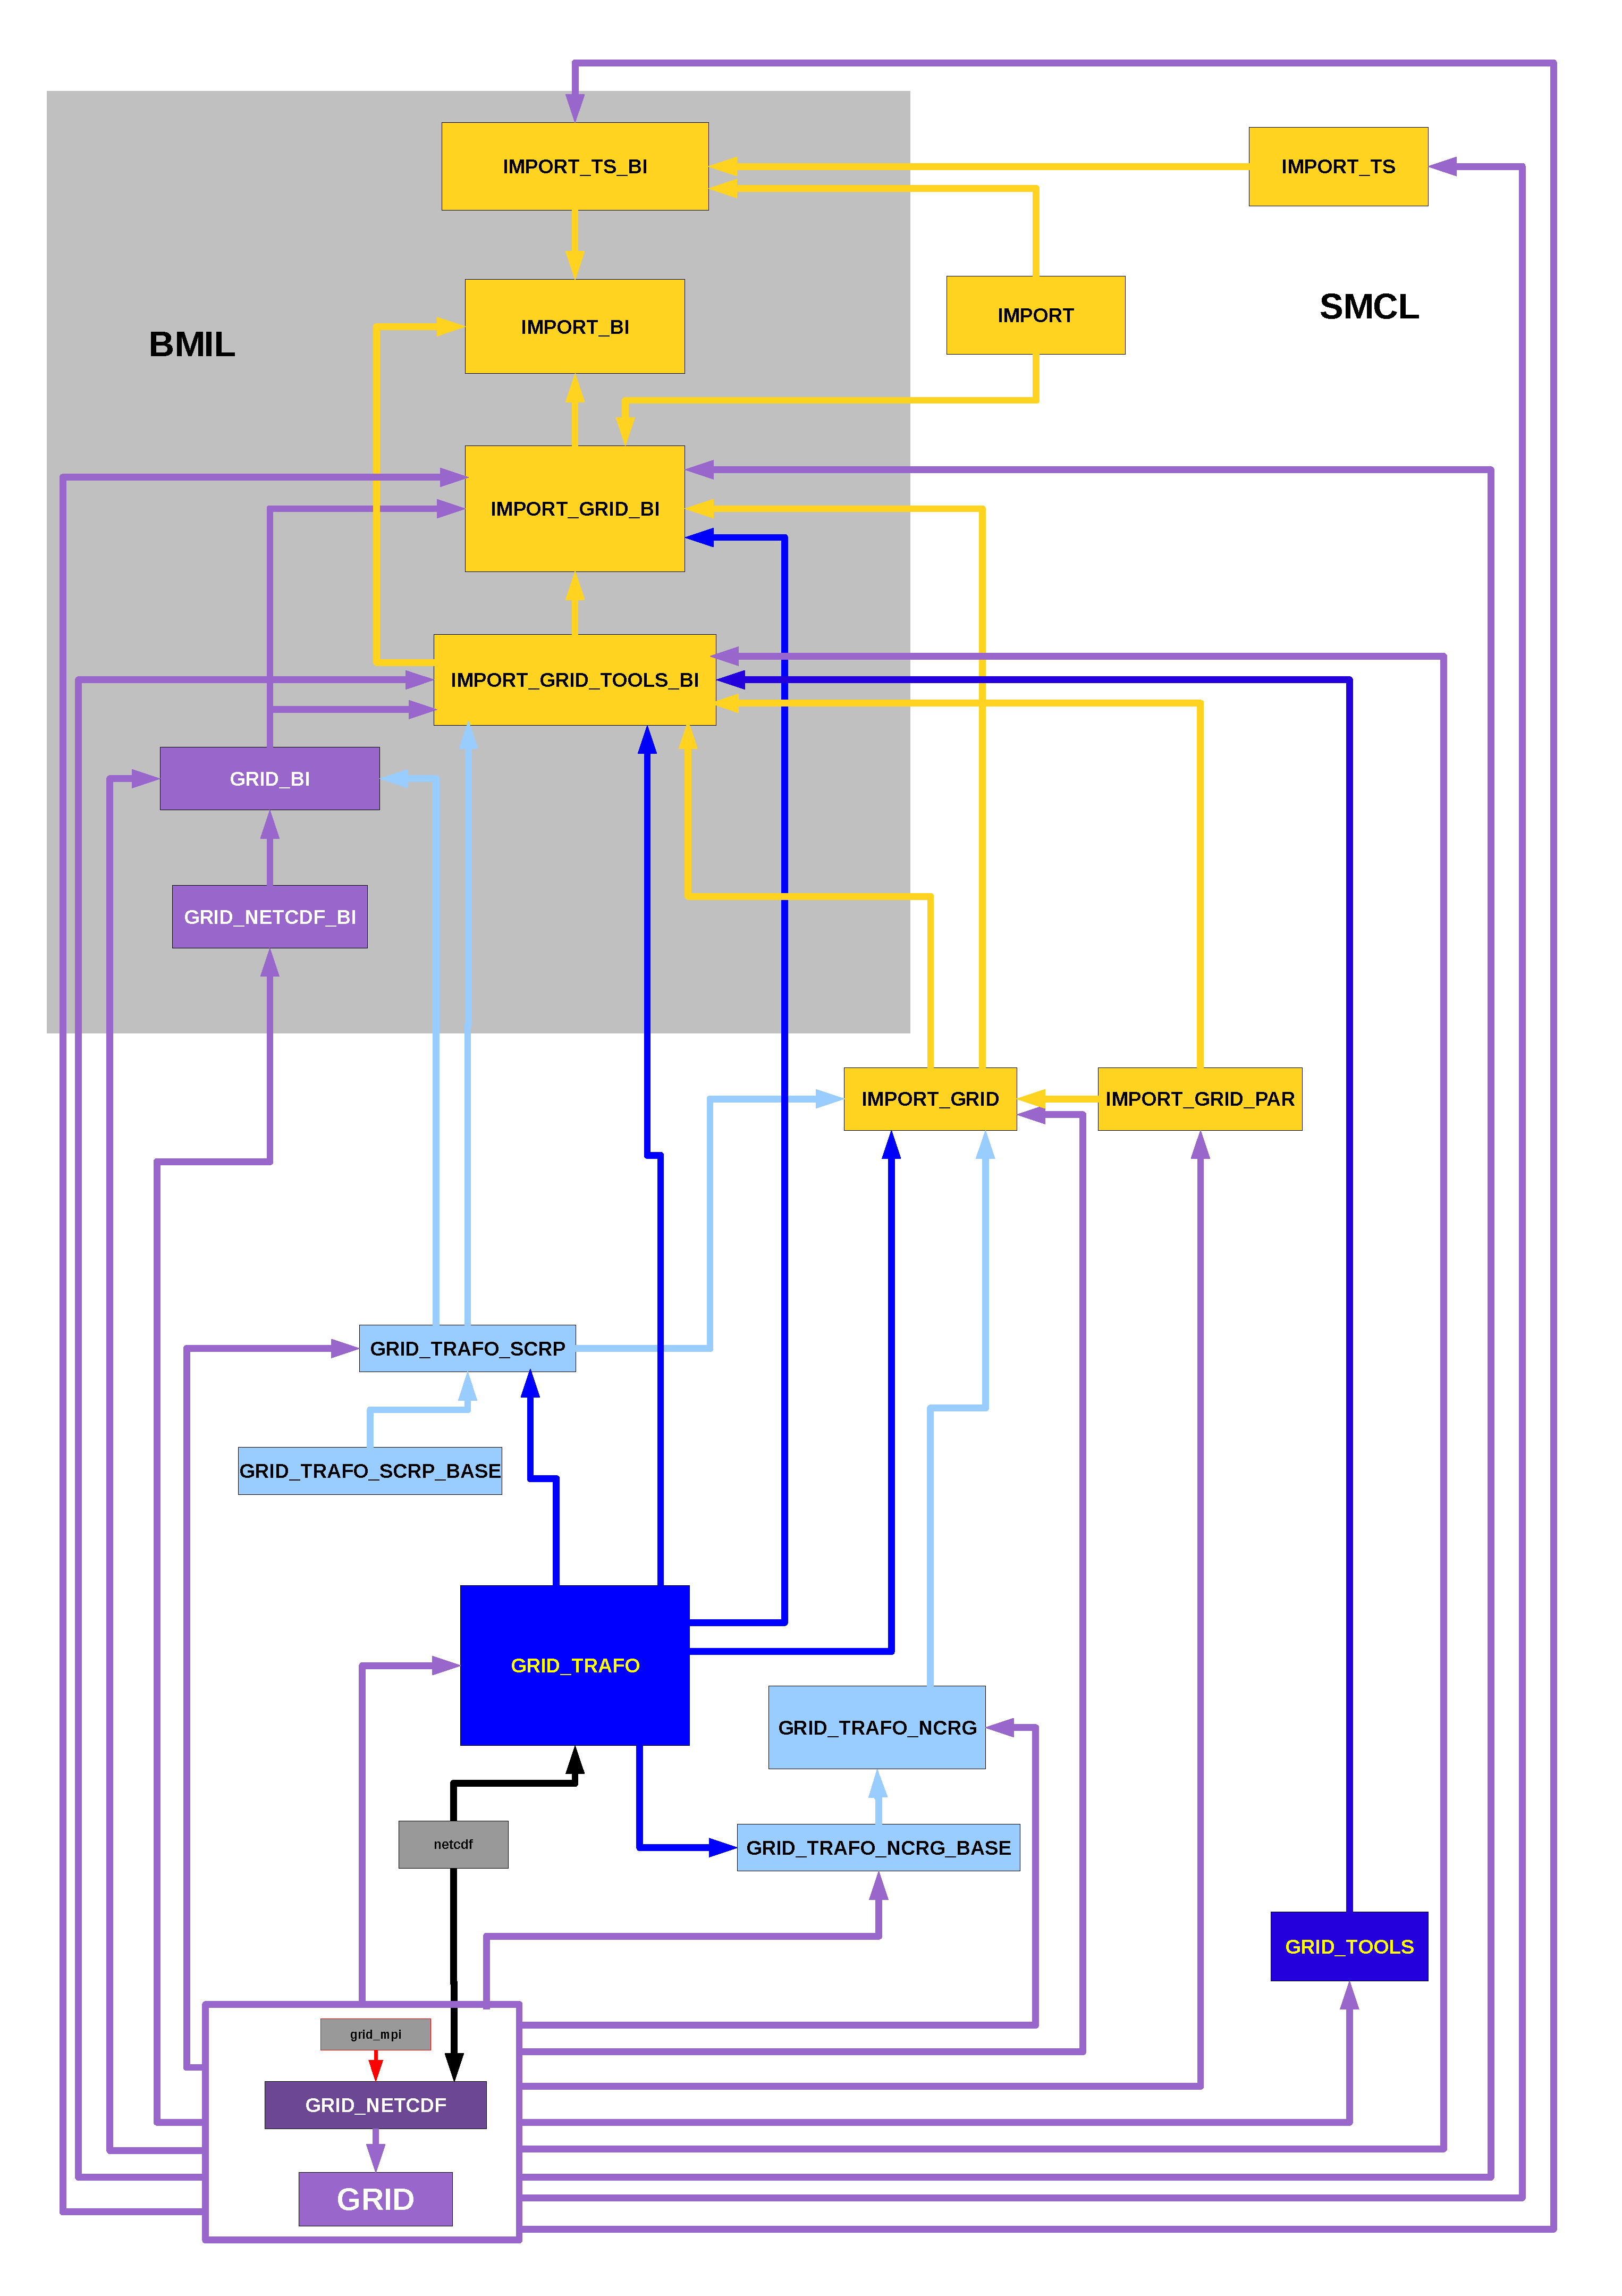
\includegraphics[height=0.87\textheight]{USEd_IMPORT.pdf}
\end{center}
\vspace*{-.5cm}
\caption{Use structure of the generic MESSy submodels GRID (bluish
colours) and IMPORT (yellow colours). The Basemodel Interface layer
(BMIL) is indicated by grey background colour. Each box equals one
module. Arrows point in the direction of the uses, e.g. the submodel
core layer (SMCL) modules are used in the BMIL. \label{USE}} 
\end{figure*}
\begin{enumerate}
\item The module \verb|MESSY_MAIN_IMPORT_GRID_BI| provides the
interface. The subroutines are called from the MESSy entry points in CONTROL
via \verb|MESSY_MAIN_IMPORT_BI|. The following MESSy entry points are
used by \verb|MESSY_MAIN_IMPORT_GRID_BI|:
\begin{itemize}
\item \verb|IMPORT_GRID_INITIALIZE|: Here the \verb|&RGTEVENTS|
namelist is read and the {\it action string}  of each
{\it regrid event} is analysed calling the
subroutine \verb|PARSE_STR|\footnote{{In subroutine \tt PARSE\_STR}
the {\it action string} is cracked into its components. This 
subroutine is located in {\tt messy\_main\_import\_grid.f90}}. \label{IGPS} 
\item \verb|IMPORT_GRID_INIT_MEMORY|: The dimensions of the
regridded data are calculated.
 For each variable imported to the model a channel object is defined.
 If attributes are associated with the
imported data, these attributes are transformed to the corresponding 
channel object attributes with the
subroutine \verb|ADD_VAR_ATTRIBUTE|.\label{IGADDATT} 
\item \verb|IMPORT_GRID_GLOBAL_START|: During the time loop 
the {\tt time\_events} of all {\it regrid events} are evaluated and,
if required, new input data is processed.
\item \verb|IMPORT_GRID_FREE_MEMORY|: At the end of the model
simulation internal memory, i.e. memory allocated in addition to the
channel objects, is released.
\end{itemize}
 
\item The module \verb|MESSY_MAIN_IMPORT_GRID_TOOLS_BI| contains the
variable declarations and routines for the {\tt time\_event}
handling. Additionally, it manages the writing / reading of the
ASCII restart file\footnote{``restart'' is here used for a user defined
checkpointing.} required to store the current status of the 
{\it counters}.
 Furthermore, it contains the interface routines which control
the import and regrid process on the basemodel interface level.
Two subroutines exist, one for the import of one specific variable
(\verb|RGTOOL_BI_READ_NCVAR|) and
one for the import of all variables hosted in one file
(\verb|RGTOOL_BI_READ_NCFILE|). 
\item The SMCL module \verb|MESSY_MAIN_IMPORT_GRID| comprises the
routines for the handling of the {\it counters} and the routines, which control
the import and regrid process on the SMCL
(\verb|RGTOOL_READ_NCVAR| and \verb|RGTOOL_READ_NCFILE|,
respectively). These routines provide the interfaces to GRID\_TRAFO
and call the respective regridding
subroutines. Furthermore, \verb|MESSY_MAIN_IMPORT_GRID|
contains the subroutine for managing the data import of the  
{\it regrid events}
(\verb|READ_CONTROL|), which itself requires the subroutines for reading the 
namelist (\verb|READ_NAMELIST|), and for parsing the information about the
variables (\verb|PARSE_VARSTR|). \label{IGPARSE}
\item The SMCL module \verb|MESSY_MAIN_IMPORT_GRID_PAR| contains
those routines required for the parallelisation of the regridding
process. For SCRIP a domain decomposition parallelisation is possible, 
i.e., each PE regrids only its subdomain.
In contrast to this, NREGRID traditionally (mainly because of the grid 
domain decomposition applied in ECHAM5) is parallelised over the
different variables (see Sect.~\ref{IGPAR}). 
\end{enumerate}
Table \ref{Tab:routines} lists the routines of IMPORT\_GRID along with
a short description. Additionally, it states the module hosting
the routine and the section in this manual providing more detailed
information on the respective routine or type.

%*************************************************************************
\subsubsection{RGTEVENT handling\label{IGevents}}
In applications of IMPORT\_GRID in interface mode, it is useful to trigger data
processing (i.e., reading / regridding of an input field) at specific
time steps (\verb|time_events|). For each of these time
steps, a specific time slice of the imported variable is used
({\it counter}).
For example, an input file contains monthly emission data, for the
years 1995 to 2003 and is used for a simulation of the year 2000.
The monthly update of the channel object is triggered by
a \verb|time_event|, while the access to the correct data for the year
2000 is managed by the {\it counter}. Both information are part of
the structure \verb|T_RGTEVENT|, which additionally includes
the {\it action string}, thus describing a {\it regrid
event}. The routines required for
the \verb|time_event| handling and the overall administration of
the \verb|RGTEVENTs| are described in the following,
 while the {\it counter} handling is described below (Sect.~\ref{IGCNT}).

\begin{longtable}{|p{5cm}p{8.5cm}cc|}
\caption{List of routines and type declarations in
IMPORT\_GRID. Routines are colored blue and structures
red. The file numbers indicate in which module the routines are
located:\\
1: MESSY\_MAIN\_IMPORT\_GRID\_BI; 2:
MESSY\_MAIN\_IMPORT\_GRID\_TOOLS\_BI; 3: MESSY\_MAIN\_IMPORT\_GRID; 
4: MESSY\_MAIN\_IMPORT\_GRID\_PAR.\label{Tab:routines}}\\
\hline
\# Routine name & Short description & file & Sect. \\
\hline
\endfirsthead
\caption{List of routines in IMPORT\_GRID (... continued)}\\
\hline
\# Routine name & Short description & file & Sect. \\
\hline
\endhead
\hline
\endfoot
%% \multicolumn{3}{l}{\bf \color{blue} MESSY\_MAIN\_IMPORT\_GRID\_TOOLS\_BI}\\
%%  & hosts routines for namelist, event and counter handling, acts as
%%  interface to the core routines
%% & \\\hline
 & & & \\ 
\multicolumn{2}{|c}{\bf \Large Interface utility routines} & & \ref{IGToolsandCore}\\ \hline%{IGevents}\\ \hline
{\color{blue} \tt PARSE\_STR} & parsing the action string of \verb|RG_TRIG|
 &  3 & \ref{IGToolsandCore}\\%{IGPS} \\ 
{\color{blue} \tt ADD\_VAR\_ATTRIBUTES} & adding the attributes defined
 during the import to the resulting channel objects
 &  1& \ref{IGToolsandCore}\\%{IGADDATT} \\ 
\hline& & & \\
\multicolumn{2}{|c}{\bf \Large RGTEVENT handling} & & \ref{IGevents}\\ \hline
{\color{red} \tt TYPE t\_rgtevent} & structure for the namelist
 variable {\tt RG\_TRIG} & 2 & \ref{IGTRGTEVENT} \\\hline
{\color{blue} \tt RGTEVENT\_INIT\_NML} & namelist reading and event
 initialisation &  2& \ref{IGRGTEVINITNML} \\ \hline
{\color{blue} \tt RGTEVENT\_STATUS} & inquiring status of {\tt
 time\_event} and updating {\it counter} &  2 & \ref{IGRGTEVSTATUS} \\\hline
{\color{blue} \tt RGTEVENT\_INIT} & initialisation of the {\tt time\_events} required for each {\it regrid event} &  2& \ref{IGRGTEVINIT} \\\hline
{\color{blue} \tt RGTEVENT\_STAT} & evaluation of the status of {\tt
 time\_event}, called from \verb|RGTEVENT_STATUS| &  2& \ref{IGRGTEVSTAT} \\\hline
{\color{blue} \tt RGTEVENT\_INDEX} & searching for the index of a specific regrid
 event  &  2& \ref{IGRGTEVINDEX} \\\hline
& & & \\
\multicolumn{2}{|c}{\bf \Large {\it Counter} handling} & & \ref{IGCNT} \\ \hline
{\color{red} \tt TYPE t\_ncrgcnt}    &  structure for the {\it counter} & 3 & \ref{IGCNTTYPE} \\\hline
{\color{blue} \tt NEW\_NCRGCNT } & creation of a new list entry in the {\it counter} list & 3 & \ref{IGCNTNEW} \\\hline
{\color{blue} \tt LOC\_NCRGCNT} & location of a specific {\it counter} in {\it counter} list  & 3 & \ref{IGCNTLOC} \\\hline
{\color{blue} \tt GET\_NEXT\_NCRGCNT} &  next element in {\it counter} list & 3 & \ref{IGCNTNEXT} \\\hline
{\color{blue} \tt RGTOOL\_NCRGCNT\_RST} & interface for {\it counter}
handling at start and restart& 3  & \ref{IGCNTRST} \\\hline
{\color{blue} \tt  NCRGCNT\_HALT} &  error flag handling & 3 & \ref{IGCNTHALT} \\\hline
{\color{blue} \tt ncrgcnt\_error\_str} &  production of an error messages & 3 & \ref{IGCNTERRSTR} \\\hline
{\color{blue} \tt CLEAN\_NCRGCNT\_LIST} &  removing all {\it counter} list entries& 3 & \ref{IGCNTLISTCLEAN} \\\hline
{\color{blue} \tt WRITE\_NCRGCNT\_LIST} &  dumping {\it counter} list to ASCII file & 3 & \ref{IGCNTLISTWRITE} \\\hline
{\color{blue} \tt READ\_NCRGCNT\_LIST} &  reading list of {\it counters} from ASCII file& 3 & \ref{IGCNTLISTREAD} \\\hline
{\color{blue} \tt \small MAIN\_IMPORT\_GRID\_WRITE\_RESTART} & calling {\tt
WRITE\_NCRGCNT\_LIST} in case of an interruption of simulation &
2 & \ref{IGWRITERST} \\\hline
{\color{blue} \tt \small MAIN\_IMPORT\_GRID\_READ\_RESTART} & calling {\tt
READ\_NCRGCNT\_LIST} in case of a resumed simulation &  2 & \ref{IGREADRST} \\\hline
{\color{blue} \tt \small IMPORT\_GRID\_TOOLS\_FREE\_MEMORY} & releasing memory of {\it counter} list &
2 & \ref{IGFREEMEM} \\\hline

%% \multicolumn{3}{l}{\bf \color{blue}  MESSY\_MAIN\_IMPORT\_GRID\_BI} \\
%%  & interface to basemodel: controls the regridding process, allocates
%%  the memory required for the imported fields & \\ \hline
%% \multicolumn{3}{l}{\bf \color{blue}  MESSY\_MAIN\_IMPORT\_GRID} \\
%%  &  controls the {\it counter}, builds interface to GRID\_TRAFO, hosts
%%  routines for file and namelist reading  & \\\hline
%% \multicolumn{3}{l}{\bf \color{blue}  MESSY\_MAIN\_IMPORT\_GRID\_PAR} \\
%%  & host important variables for the parallelisation of the data import  & \\\hline
%% {
& & & \\
\multicolumn{2}{|c}{\bf \Large The importing routines}
& & \ref{IGREAD} \\ \hline
{\color{blue} \tt READ\_NAMELIST} & reading the regridding namelist &
3 & \ref{IGREADNML} \\\hline
{\color{blue} \tt PARSE\_VARSTR} & parsing the variable string
(\tt var=...) &
3 & \ref{IGPARSEVARSTR} \\\hline
{\color{blue} \tt RGTOOL\_READ\_NCVAR} &  import and regridding of a single
variables & 3 & \ref{RGREADNCVAR} \\\hline
{\color{blue} \tt RGTOOL\_READ\_NCFILE} &  import and regridding of all
variables of one data file & 3 & \ref{RGREADNCFILE} \\\hline
{\color{blue} \tt READ\_CONTROL} &  data import by reading the
regridding namelists and afterwards importing the data from the file & 3 & \ref{IGREADCONTROL} \\\hline
& & & \\
\multicolumn{2}{|c}{\bf \Large Parallelisation}
& & \ref{IGPAR} \\ \hline
{\color{red} \tt t\_mpi\_def} & information of parallel
environment & 4 &\ref{IGtypeMPI}\\ \hline
{\color{blue} \tt DISTRIBUTE\_VARS\_ON\_PES} &  parallelisation along
variable space &  4 & \ref{IFDVOPE} \\\hline
{\color{blue} \tt INIT\_PNCREGRID} & initialisation of variables used for
parallelisation & 4  & \ref{IGPARINITPNCREGRID} \\\hline
{\color{blue} \tt INIT\_PARALLEL} & collecting information of parallel environment &
4 & \ref{IGPARINIT} \\\hline
{\color{blue} \tt EXPAND\_FILENAME} & expanding the output filename by PE number in case of
parallelisation &  4 & \ref{IGPAREXPFILENAME} \\\hline
\end{longtable}
\vspace*{0.5cm}
%main_import_grid_tools_bi


\paragraph{\color{red} \tt\bf TYPE T\_RGTEVENT\\\label{IGTRGTEVENT}}

For the handling of the {\it regrid events} the type 
\verb|T_RGTEVENT| hosting the event information is defined:
\begin{verbatim}
  ! USED FOR NAMELIST-INPUT
  TYPE T_RGTEVENT_IO
     TYPE(io_time_event)         ::  &
                   evt = io_time_event(1, TIME_INC_MONTHS,TRIG_EXACT,0)
     TYPE(T_NCRGCNT)             :: cnt = T_NCRGCNT('', -1, -1, -1, -1)
     CHARACTER(LEN=RGTMAXACTSTR) :: act = ''
  END TYPE T_RGTEVENT_IO

  ! INTERNAL WORKSPACE
  TYPE T_RGTEVENT
     TYPE(T_RGTEVENT_IO) :: io
     TYPE(time_event)    :: event
  END TYPE T_RGTEVENT
\end{verbatim}
 Type \verb|T_RGTEVENT| consists of the corresponding structure
 component of type \verb|T_RGTEVENT_IO| used for 
 the namelist input of the {\it regrid event}, and an internally used
 \verb|time_event| (see TIMER 
User Manual). The  type \verb|T_RGTEVENT_IO| contains the structure
 components described above: the \verb|io_time_event|, the {\it counter}
 (type \verb|T_NCRGCNT|) and the {\it  action string}. 
For the definition of the {\it counter} see Sect.~\ref{IGCNT}.\\

\paragraph{SUBROUTINE \color{blue} \tt\bf RGTEVENT\_INIT\_NML\\ \label{IGRGTEVINITNML}}
The \verb|&RGTEVENTS| namelist is read in this subroutine by
calling the  
private subroutine \verb|RGTEVENT_READ_NML_CPL| on the I/O-PE and 
afterwards broadcasted
to all PEs. Additionally, the individual \verb|time_event|s are
initialised via subroutine \verb|RGTEVENT_INIT|, followed directly by
the investigation of the 
{\it regrid event} status by calling the subroutine \verb|RGTEVENT_STATUS|.\\

\paragraph{SUBROUTINE \color{blue} \tt\bf RGTEVENT\_STATUS\\ \label{IGRGTEVSTATUS}}

The interface of the subroutine \verb|RGTEVENT_STATUS|  is defined by
\begin{verbatim}
! ------------------------------------------------------------------
SUBROUTINE RGTEVENT_STATUS(status, cpos, rgt, modstr, name, index, action &
                          , lstop, linit)

  ! RETURNS THE EVENT STATUS (flag) OF A NAMED (name)
  ! OR INDEXED (index) RGT-EVENT IN A LIST (rgt)
  !
  ! Author: Patrick Joeckel, MPICH, Mainz, October 2002

  ...

  IMPLICIT NONE
  ...

  ! I/O
  LOGICAL,                      INTENT(OUT)            :: status ! event status
  INTEGER,                      INTENT(OUT)            :: cpos   ! counter pos. 
  TYPE(T_RGTEVENT), DIMENSION(:), POINTER              :: rgt    ! RGT-event list
  CHARACTER(LEN=*),             INTENT(IN)             :: modstr ! calling module
  CHARACTER(LEN=*),             INTENT(IN),  OPTIONAL  :: name   ! name of event
  INTEGER,                      INTENT(IN),  OPTIONAL  :: index  ! index of event
  CHARACTER(LEN=RGTMAXACTSTR),  INTENT(OUT), OPTIONAL  :: action ! action string
  LOGICAL,                      INTENT(IN),  OPTIONAL  :: lstop  ! stop on error
  LOGICAL,                      INTENT(IN),  OPTIONAL  :: linit  ! initialize?
! ------------------------------------------------------------------
\end{verbatim}
The status of the \verb|time_event| is calculated using the
subroutine \verb|RGTEVENT_STAT|. Secondly, the {\it counter} of the
{\it regrid event}  is updated using subroutine \verb|RGTOOL_NCRGCNT_RST|.
Last but not least, the output parameters, i.e., the current position
of the {\it counter} (\verb|cpos|) and the \verb|status| flag are
set. If the {\it action string} is 
requested, it is copied to the optional parameter \verb|action|.

For identification of the respective {\it regrid event},
the \verb|name| or the  \verb|index| are required. If both are not
present the returned status is non-zero. If only the \verb|name| is
provided, the \verb|index| is obtained by calling the 
subroutine \verb|RGTEVENT_INDEX|. If no {\it regrid event} with the
provided \verb|name| 
is found, the returned status flag is non-zero. The same happens, if the given
index is not available in the list of  {\it regrid event}s. 
Note: if the \verb|index| is provided during the subroutine call, the
value of   
\verb|name| is ignored. There is no internal test, if \verb|name|
and  \verb|index| fit.
 
\paragraph{SUBROUTINE \color{blue} \tt\bf RGTEVENT\_INIT\\ \label{IGRGTEVINIT}}
This subroutine performs the initialisation of the \verb|time_event|s
corresponding to the {\it regrid events}.%\footnotemark[\ref{TUM}].
\paragraph{SUBROUTINE \color{blue} \tt\bf RGTEVENT\_STAT\\ \label{IGRGTEVSTAT}}
This subroutine evaluates the status of a {\tt
time\_event} %\footnotemark[\ref{TUM}] 
by calling the TIMER function \verb|event_state|.
\paragraph{SUBROUTINE \color{blue} \tt\bf RGTEVENT\_INDEX\\ \label{IGRGTEVINDEX}}
This subroutine searches the list of {\it regrid events} to locate
the \verb|index| of a {\it regrid event} of a specific name.
%%MESSY\_MAIN\_IMPORT\_GRID
%*************************************************************************
\subsubsection{{\it Counter} handling\label{IGCNT}}
This subsection describes how the {\it counter} information is processed.
For this, \verb|MESSY_MAIN_IMPORT_GRID|
contains an additional type declaration, and the corresponding subroutines to
provide this functionality.
\paragraph{\color{red} \tt\bf TYPE T\_NCRGCNT\\ \label{IGCNTTYPE}}
The type \verb|T_NCRGCNT| provides a structure to store {\it counter} information:
\begin{verbatim}
TYPE T_NCRGCNT
  CHARACTER(LEN=NCCNTMAXNLEN) :: name    = ''
  INTEGER                     :: start   = 1
  INTEGER                     :: step    = 1
  INTEGER                     :: reset   = 1
  INTEGER                     :: current = 1
END TYPE T_NCRGCNT
\end{verbatim}
\verb|name| is used to identify the {\it counter} (e.g., in a list of {\it counters}), 
\verb|start| contains the minimum {\it counter} position, \verb|step| the increment,
 and \verb|reset| the maximum {\it counter} position. The current {\it counter} position
can for instance be used to read / regrid a
specific time step of a netCDF variable by setting the parameter \verb|t| of
subroutine \verb|RGTOOL_READ_NCVAR| or subroutine
\verb|RGTOOL_READ_NCFILE| to \verb|current| 
(see Sect.~\ref{IGREAD}).

To process a large number of {\it counters} the individual {\it
counters} are stored in a concatenated list:
\begin{verbatim}
  TYPE T_NCRGCNT_LIST
     CHARACTER(NCCRSTRL)           :: mname  = ''
     TYPE(T_NCRGCNT)               :: this
     TYPE(T_NCRGCNT_LIST), POINTER :: next => NULL()
  END TYPE T_NCRGCNT_LIST
\end{verbatim}
\verb|mname| is the name of the submodel defining this {\it counter}.

\paragraph{SUBROUTINE \color{blue} \tt\bf NEW\_NCRGCNT\\ \label{IGCNTNEW}}
With this subroutine a new list entry in the concatenated list of {\it counters}
is created. 
\begin{verbatim}
! ------------------------------------------------------------
  SUBROUTINE new_ncrgcnt(status, mname, cnt)

    IMPLICIT NONE

    ! I/O
    INTEGER,          INTENT(OUT)  :: status
    CHARACTER(LEN=*), INTENT(IN)   :: mname
    TYPE(t_ncrgcnt),  INTENT(IN)   :: cnt
! ------------------------------------------------------------
\end{verbatim}
Input to the subroutine is a {\it counter} of type \verb|T_NCRGCNT|
and the name 
\verb|mname| of the submodel defining the {\it counter},
i.e., \verb|'import_grid'|. 
(This option is a relict of earlier versions without unique interface
for data import into a MESSy model: all submodels importing data had
to include there own interface to NCREGRID. In this case it was
important to know, which submodel defined the respective {\it counter}).
 A \verb|status| flag is handed back to the calling routine providing 
information about errors or the information, if a {\it counter}
already exists. 

\paragraph{SUBROUTINE \color{blue} \tt\bf LOC\_NCRGCNT\\ \label{IGCNTLOC}}
This subroutine locates a {\it counter} in the concatenated list:
\begin{verbatim}
  ! -------------------------------------------------------------------
  SUBROUTINE loc_ncrgcnt(status, mname, cname, cntptr)

    IMPLICIT NONE

    ! I/O
    INTEGER,              INTENT(OUT) :: status
    CHARACTER(LEN=*),     INTENT(IN)  :: mname
    CHARACTER(LEN=*),     INTENT(IN)  :: cname
    TYPE(t_ncrgcnt),      POINTER     :: cntptr
  ! -------------------------------------------------------------------
\end{verbatim}
The name of the defining submodel (\verb|mname|) and the {\it counter} name 
 (\verb|cname|) are input to the routine. If the {\it counter} is found, the 
pointer \verb|cntptr| is associated to the {\it counter} and the \verb|status|
is zero. Otherwise, the pointer \verb|cntptr| is NULLIF(Y)ied and the 
 \verb|status| flag provides information about the reason: 

\begin{tabular}{ll}
status  &  error \\ \hline 
5003    &  {\tt mname} too long \\
5006  &  {\tt cname} too long \\
5005 & {\it counter} does not exist\\ \hline
\end{tabular}

\paragraph{SUBROUTINE \color{blue} \tt\bf GET\_NEXT\_NCRGCNT\\ \label{IGCNTNEXT}}
The subroutine \verb|GET_NEXT_NCRGCNT| can be used to loop over all 
currently stored {\it counters} in the internal list, e.g., to search for a 
specific {\it counter}:
\begin{verbatim}
 LOGICAL                  :: last 
 TYPE(t_ncrgcnt), POINTER :: cptr
   ...
 DO
   CALL GET_NEXT_NCRGCNT(last, cptr)
   IF (last) EXIT
   ! check cptr here
   ....
 END DO
\end{verbatim}
\verb|last| is \verb|.TRUE.|, if the end of the list is reached. 
This construction is required, since the number of {\it counters}
stored in the internal list is not known a priori.
Internally the subroutine distinguishes two modes: \verb|MODE_INIT|
and \verb|MODE_CONT|. At the first call, the \verb|MODE| is set
to \verb|MODE_INIT|. This triggers that the internal pointer is set to
the start element of the concatenated list of {\it counters}
(\verb|GRGTLIST)|. Afterwards the \verb|MODE| is set
to \verb|MODE_CONT|. If the first list element exists, this pointer is
returned and \verb|MODE| is still \verb|MODE_CONT|, so that at
the next call of the subroutine the next pointer in the list can be
accessed.

\begin{verbatim}
! -------------------------------------------------------------------
  SUBROUTINE GET_NEXT_NCRGCNT(last, cntptr)

    IMPLICIT NONE

    ! I/O
    LOGICAL,              INTENT(OUT) :: last
    TYPE(t_ncrgcnt),      POINTER     :: cntptr
! -------------------------------------------------------------------
\end{verbatim}
As long as more list elements exist, upon return, \verb|cntptr| is
associated to  
the next element and \verb|last| is set \verb|.FALSE.|. If no more elements
are available, \verb|last| is set \verb|.TRUE.| and \verb|cntptr| keeps its
association. Additionally \verb|MODE| is reset to \verb|MODE_INIT|,
indicating that at the next call of the
subroutine \verb|GET_NEXT_NCRGCNT| the cycling of  
the concatenated list must start at the very beginning of the list.


\paragraph{SUBROUTINE \color{blue} \tt\bf RGTOOL\_NCRGCNT\_RST\\ \label{IGCNTRST}}
This subroutine provides an interface for the automatic handling of
 {\it counter}  information, including
\begin{itemize}
\item the update of the {\it counter} (triggered
 by \verb|event==.TRUE.|): The actual  {\it counter} position 
\verb|current| is incremented by \verb|step|. If the result is larger
than  \verb|reset|, 
  \verb|current| is reset to  \verb|start|. This allows cyclic counting.
\item the unambiguous storage of a specific {\it counter} in the
concatenated list of all {\it counters} (triggered
 by \verb|linit==.TRUE.|). This makes the {\it counter}
accessible from everywhere, which is required to save the {\it
counters} in an external file at model interruption during a user defined
 checkpointing (restart). 
\item the continuous update of the actual {\it counter} and its
 copy stored in the concatenated central list.
\end{itemize}
The subroutine is called with the following parameters:
\begin{verbatim}
! ----------------------------------------------------------------------
  SUBROUTINE RGTOOL_NCRGCNT_RST(mname, start, restart, event, c, lout, linit)

    ! MANAGES I/O OF COUNTER INFORMATION AT START AND RESTART
    !
    ...

    IMPLICIT NONE

    INTRINSIC :: PRESENT, TRIM

    ! I/O
    CHARACTER(LEN=*), INTENT(IN)    :: mname
    LOGICAL,          INTENT(IN)    :: start   ! .true. at first time step
    LOGICAL,          INTENT(IN)    :: restart ! .true. at first time step of
                                               ! rerun
    LOGICAL,          INTENT(IN)    :: event   ! .true. on event
    TYPE(T_NCRGCNT),  INTENT(INOUT) :: c       ! counter - struct
    LOGICAL,          INTENT(IN)    :: lout
    LOGICAL,OPTIONAL, INTENT(IN)    :: linit

! ----------------------------------------------------------------------
\end{verbatim}
\begin{itemize}
\item \verb|mname| is a name identifying the defining submodel.
\item \verb|start| must be \verb|.TRUE.| only at the very first model
    time step. It is used to prevent a {\it counter} 
update immediately at model start, if at the same time the event is triggered.
\item \verb|restart| must be \verb|.TRUE.| only after the first
initialisation of the {\it counter} list from the restart file. 
This is used to restore the actual {\it counter} from the list,
even if the event is not triggered.
\item \verb|event| is \verb|.TRUE.|, indicating that the {\it counter} update is triggered.
\item \verb|c| is the {\it counter} structure of the actual {\it counter}.
\item \verb|lout| is \verb|.TRUE.| for diagnostic output.
\item \verb|linit| is an optional switch (default: .\verb|FALSE.|). 
If set to \verb|.TRUE.|, it prevents {\it counters} of the same name and 
\verb|mname| to be updated, if the {\it counter} exists already in the
list, but creates a new entry in the {\it counter} list, if it is
new. This is required to enable the definition of additional {\it
regrid events} after restart.
\end{itemize}
The sequence of operations is as follows:
\begin{enumerate}
\item If \verb|start|, \verb|restart|, and \verb|event| are all 
\verb|.FALSE.|, the subroutine is left immediately.
\item The algorithm locates the specified {\it counter} \verb|c| by
its name and \verb|mname|.
If the {\it counter} is found, the content of the respective {\it
counter} in the list is copied to the actual {\it counter} \verb|c|.
\item The initialisation flag \verb|linit| is checked: Only if \verb|linit|
 is \verb|.TRUE.| the presence of the {\it counter} in the list is
 re-evaluated:  
If it exists in the list, the routine returns with a non-zero error
 status, since during the initialisation, the {\it counter} must not yet
exist. If the {\it counter} is new, however, it is added to the list.
\item The algorithm checks, if an update has been triggered. Only if 
\verb|event| is \verb|.TRUE.| and \verb|start| is \verb|.FALSE.|,
 an existing actual {\it counter} and its copy in the
central list are updated, as described above. If the {\it counter}
does not exist in the list, the routine exits with a non-zero status.
\end{enumerate}

\paragraph{SUBROUTINE \color{blue} \tt\bf NCRGCNT\_HALT\\ \label{IGCNTHALT}} 

\par\noindent This routine provides the handling of the error status flags delivered by other subroutines.
It uses the RMSG subroutine from GRID to stop the simulation, if an
error occurs.
\begin{verbatim}
 ! ------------------------------------------------------------------
  SUBROUTINE ncrgcnt_halt(substr, status)

    ! MESSy
    USE messy_main_constants_mem,  ONLY: STRLEN_VLONG
    USE messy_main_grid_netcdf,    ONLY: RGMSG, RGMLE
    
    IMPLICIT NONE
    ! I/O
    CHARACTER(LEN=*), INTENT(IN)  :: substr
    INTEGER,          INTENT(IN)  :: status
 ! ------------------------------------------------------------------
\end{verbatim}
Input to the subroutine are a character string (\verb|substr|) indicating
the calling routine and the \verb|status| flag to be evaluated.

\paragraph{FUNCTION \color{blue} \tt\bf ncrgcnt\_error\_str\\ \label{IGCNTERRSTR}}
This function provides a meaningful error string associated to the respective status flag.
It is used by subroutine \verb|NCRGCNT_HALT|.

\paragraph{SUBROUTINE \color{blue} \tt\bf CLEAN\_NCRGCNT\_LIST\\ \label{IGCNTLISTCLEAN}}
This subroutine is used to remove all
{\it counter} list entries, i.e., to clean up the memory.

\paragraph{SUBROUTINE \color{blue} \tt\bf WRITE\_NCRGCNT\_LIST\\\label{IGCNTLISTWRITE}}
With the subroutine \verb|WRITE_NCRGCNT_LIST| the complete
 concatenated list of currently stored {\it counter} information is
 dumped into an ASCII file. This is required for restarts.
\paragraph{SUBROUTINE \color{blue} \tt\bf READ\_NCRGCNT\_LIST\\ \label{IGCNTLISTREAD}}
With subroutine \verb|READ_CRGCNT_LIST|, the {\it counter} information
is restored from a file previously written by
subroutine \verb|WRITE_NCRGCNT_LIST|. This is required for restarts.
%tools_bi
\paragraph{SUBROUTINE \color{blue} \tt\bf MAIN\_IMPORT\_GRID\_WRITE\_RESTART\\ \label{IGWRITERST}}
This BMIL subroutine calls the SMCL routine \verb|WRITE_NCRGCNT_LIST|,
if writing of restart files is triggered. 
\paragraph{SUBROUTINE \color{blue} \tt\bf MAIN\_IMPORT\_GRID\_READ\_RESTART\\ \label{IGREADRST}}
This BMIL subroutine calls the SMCL routine \verb|READ_NCRGCNT_LIST|,
if a simulation is resumed after restart.
\paragraph{SUBROUTINE \color{blue} \tt\bf IMPORT\_GRID\_TOOLS\_FREE\_MEMORY\\ \label{IGFREEMEM}}
This BMIL subroutine initiates the initialisation of the concatenated
list of {\it counters} by calling the SMCL routine \verb|CLEAN_NCRGCNT_LIST|.


%*************************************************************************
\subsubsection{Interfaces for file reading and regridding\label{IGREAD}}
%main_import_grid_tools_bi
The SMCL file \verb|MESSY_MAIN_IMPORT_GRID| contains all subroutines
 managing the data import and regridding.
The subroutines \verb|RGTOOL_READ_NCVAR| and 
\verb|RGTOOL_READ_NCFILE| are the drivers of these processes for import of
single variables (\verb|NCVAR|), or all variables contained in one file 
(\verb|NCFILE|), respectively. The corresponding BMIL interfaces are
the subroutines \verb|RGTOOL_BI_READ_NCVAR| and  
\verb|RGTOOL_BI_READ_NCFILE|, respectively, located
in \verb|MESSY_MAIN_IMPORT_GRID_TOOLS_BI|.  

\paragraph{Subroutines {\color{blue} \tt\bf RGTOOL\_BI\_READ\_NCVAR} and
{\color{blue} \tt\bf RGTOOL\_BI\_READ\_NCFILE}\\}
These two subroutines provide the main entry points on the BMIL of
IMPORT\_GRID and internally call the corresponding SMCL routines, which
acutally do the reading and regridding of the input data and the main 
IMPORT\_GRID BMIL. After processing the data, the format of  the
data is converted from the internal 1D vector to the 4D arrays 
corresponding to the respective representation. This
conversion is performed by the GRID subroutine \verb|RGTOOL_CONVERT|. 
Here especially the order of the ranks in the
4D arrays is important. Additionally, if the processing is not
performed in parallel mode and a new grid has been created by the 
SMCL routines, this grid is broadcasted to all PEs.
 In case of parallel domain decomposed input 
(\verb|ldompar =.TRUE.|) each PE hosts its own sub-grid definition.
 
%%MESSY\_MAIN\_IMPORT\_GRID
\paragraph{SUBROUTINE \color{blue} \tt\bf RGTOOL\_READ\_NCVAR\\ \label{RGREADNCVAR}}

This subroutine manages the import and the regridding of the data for single
variables. The interface is given by:
\begin{verbatim}
  SUBROUTINE RGTOOL_READ_NCVAR(status, iou, nmlfile, vname, t, var   &
                              , iipol, ogridid, igridid, SCRIP_ID    &
                              , lrg, lrgx, lrgy, lrgz, lok , oarea   &
                              , convgrid, ldompar, lvarpar)
\end{verbatim}
The meaning of the individual arguments is briefly described in Table \ref{TabReadNCVAR}.
The subroutine starts with the initialisation of local variables
controlled by the optional arguments. 
First the output grid structures (\verb|conv_grid| and \verb|ogrid|)
are initialised.  
These two grids are different, if the subroutine 
\verb|RGTOOL_READ_NCVAR| is used to simply read the input field. 
Additionally, the structure \verb|var| containing the read or
 regridded field is initialised.
As in principle, the namelist file of one {\it regrid event} can contain
any number of \verb|&RGTEVENT| namelists, an endless DO-loop builds
 the main part of 
the subroutine. To control the cycling conditions three internal
 parameters are used:
\begin{itemize}
\item \verb|RG_CTRL|:  
\begin{itemize}
\item \verb|RG_SCAN|: scan the namelist
\item \verb|RG_PROC|: process data
\item \verb|RG_STOP|: stop data processing and namelist scanning
\end{itemize} 
\item \verb|RG_NML|:   
\begin{itemize}
\item \verb|NML_NEXT|: read next namelist
\item \verb|NML_STAY|: read namelist again and import data
\end{itemize} 
\item \verb|RG_STATUS|: 
\begin{itemize}
\item \verb|RGSTAT_START|: start regridding procedure
\item  \verb|RGSTAT_CONT|: continue endless DO-loop
\item \verb|RGSTAT_STOP|: exit endless DO-loop
\end{itemize} 
\end{itemize}
\begin{table}[b]
{\footnotesize
\begin{tabular}{llllp{7.5cm}}
variable & INTENT & \multicolumn{2}{l}{type} & meaning \\ \hline
\verb|status|  & OUT & INTEGER & &status flag for GRID routines (0 = ok, if /= 0 information is provided via function \verb|grid_error|)\\
\verb|iou|     & IN  & INTEGER & &I/O unit \\
\verb|nmlfile| & IN  & CHARACTER & &namelist filename\\
\verb|vname|   & IN  & CHARACTER & &name of the variable to process \\
\verb|t|     & IN  & INTEGER & &times step in netCDF file\\
\verb|var|   & OUT  & TYPE(\verb|t_ncvar|)& & out structure \\
\verb|iipol| & IN  & INTEGER & &interpolation method (one of \verb|GTRF_NONE|, \verb|GTRF_SCRP| or \verb|GTRF_NRGT|)\\
\verb|ogridid|     & IN  & INTEGER & & ID of destination grid \\
\verb|igridid|     & INOUT  & INTEGER& & ID of source (netCDF file) grid  \\
\verb|SCRIP_ID|     & INOUT  &INTEGER & &ID of SCRIP structure \\
\verb|lrg|     & IN  & LOGICAL& OPTIONAL  & flag for interpolation. If .FALSE. data is only read in.\\
\verb|lrgx|     & IN  & LOGICAL & OPTIONAL  &  flag for interpolation in first horizontal (x-)direction\\
\verb|lrgy|     & IN  & LOGICAL & OPTIONAL  &  flag for interpolation in second horizontal \mbox{(y-)direction}\\
\verb|lrgz|     & IN  & LOGICAL & OPTIONAL  &  flag for vertical interpolation\\
\verb|lok|     & OUT  & LOGICAL & OPTIONAL &  success flag for subroutine (\verb|lok = .TRUE.| includes \verb|status == 0|, but not the other way round.)\\
\verb|oarea|     & IN  & REAL(dp) & OPTIONAL & area of zells in output grid, might be used in SCRIP\\
\verb|conv_grid|     & INOUT  & TYPE(\verb|t_geohybgrid|)& OPTIONAL &
grid structure, which is required for grid conversions in the interface subroutine \verb|RGTOOL_BI_READ_NCVAR| \\
\verb|ldompar|     & IN  & LOGICAL & OPTIONAL &  parallelisation over the destination domain\\
\verb|lvarpar|     & IN  & LOGICAL &  OPTIONAL & parallelisation over
variables  \\ \hline
\end{tabular}
}
\caption{List of arguments of subroutine {\tt RGTOOL\_READ\_NCVAR}\label{TabReadNCVAR}}
\end{table}

Start values at the  beginning of the endless loop
 are \verb|RG_CTRL=RG_SCAN|, 
 as the namelist file has to be scanned for the required namelist entry, and
\verb|RG_NML=RG_NEXT| as the next namelist should be read.
Figure \ref{FigREADNCVAR} illustrates the flow of the subroutine 
\verb|RGTOOL_READ_NCVAR|.
\begin{figure}
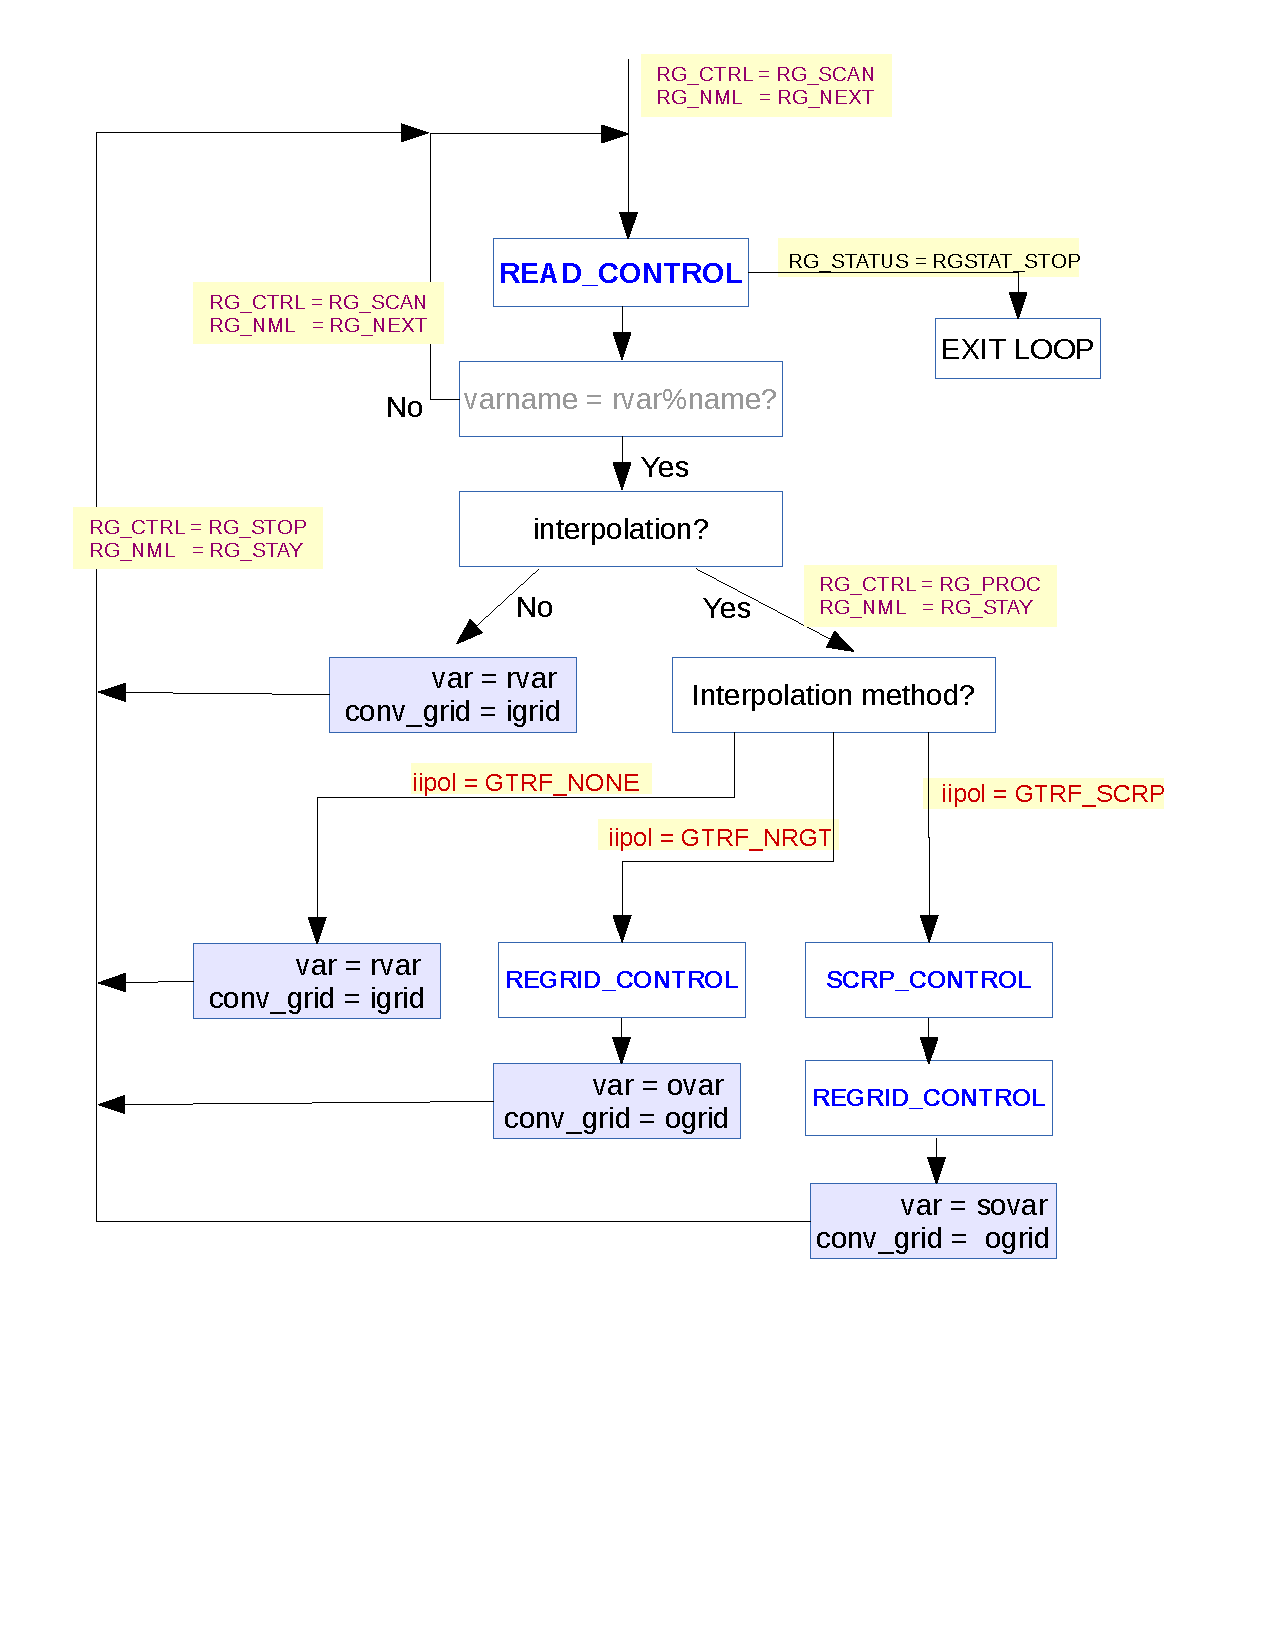
\includegraphics[width=\textwidth]{flxdiagREAD_NCVAR.pdf}
\vspace*{-4.7cm}
\caption{Flux diagram for endless DO-loop in subroutine {\tt RGTOOL\_READ\_NCVAR}. Blue letters indicate subroutine calls, the light yellow boxes show settings
of the internal switches.\label{FigREADNCVAR}}
\end{figure}
First in the endless DO-loop, the subroutine  \verb|READ_CONTROL| is called.
In that subroutine, depending on the switches  \verb|RG_CTRL| and  
\verb|RG_NML|, a namelist and the required data are read (see
Sect.~\ref{IGREADCONTROL}). 
After exiting the subroutine \verb|READ_CONTROL|, it is checked whether the
currently read namelist entry (variable name) is the requested variable.
If not,  \verb|RG_CTRL| and \verb|RG_NML| are set to \verb|RG_SCAN| and
 \verb|RG_NEXT|, respectively, and the endless DO-loop cycle starts 
again.
If the required variable has been found, the data is processed
according to \verb|llrg|:
\begin{itemize}
\item {\tt llrg=.FALSE.:} In the initialisation phase of the model,
i.e., for dimensioning the output data (\verb|channel objects|),
the namelists are read once, 
without starting the remapping. Thus, \verb|llrg| is set \verb|.FALSE.|
  in the initialisation phase. In this case, only raw data input is required. 
\verb|RG_CTRL| is set to \verb|RG_SCAN| and the imported raw data
(local structure \verb|rvar|) is copied to the output structure \verb|var|.
Additionally, the input grid specifications are added to the list of
 geo-hybrid grids by calling the GRID subroutine \verb|NEW_GEOHYBGRID|. 
Furthermore, if the data set should be regridded by SCRIP, the SCRIP 
interpolation weights are calculated and stored
in the respective data structures. Last but not least, the input grid is copied
to the output structure \verb|conv_grid| for the dimensioning of the
output structures.
\item  {\tt llrg=.TRUE.:} This signifies (usually during the time loop) that
regridding of the imported raw data is requested.  
In this case, \verb|RG_CTRL| is set to \verb|RG_PROC|. 
Depending on the chosen method, the data is regridded:
\begin{itemize}
\item \verb|GTRF_NONE|: If no grid transformation is requested, the
raw data is copied to the output structure \verb|var| and the input
grid is copied to the output grid structure \verb|conv_grid|.
\item \verb|GTRF_NRGT|: If regridding by NREGRID is chosen, 
\verb|REGRID_CONTROL| is called (see GRID-User-Manual). Afterwards, the
regridded structure \verb|ovar| is copied to the output structure \verb|var|
and the destination grid is copied to \verb|conv_grid|.
\item \verb|GTRF_SCRP|: This is the most complex call, as SCRIP
transforms only horizontal grids. Thus, first it is checked, if
horizontal regridding is requested (\verb|llrgx=.TRUE.| and /
or \verb|llrgy=.TRUE.|). In this case, 
\verb|SCRIP_CONTROL| is called, otherwise the raw data
is copied to the intermediate structure \verb|sovar|.
If vertical grid transformation is requested, NREGRID is used.
In this case, the grid specification has to be adapted to the horizontally 
regridded data. This is especially important for data on curvi-linear grids,
as NREGRID can not deal with this. As NREGRID is only used for the vertical
grid transformation, the horizontal grid is defined in a way, that
NREGRID can handle it.
A simple example: For the COSMO model grid, the coordinates of the
horizontal grid  
are defined in the rotated coordinate system. This grid is  
``pseudo-geographically-rectangular'' and not curvi-linear and NREGRID can
deal with it.
After redefining the input grid, \verb|REGRID_CONTROL| is called with the 
arguments \verb|llrgx=.FALSE.| and \verb|llrgy=.FALSE.|, as the horizonal
mapping was already performed by SCRIP.
After the vertical grid transformation, the output structures \verb|var| and
\verb|conv_grid| are filled.
\end{itemize}
\end{itemize}
After processing, \verb|RG_CTRL| is set to \verb|RG_STOP| and some 
local structures and variables are reinitialised to free the memory.
In the next call of \verb|READ_CONTROL| some further internally
allocated memory is released and the endless DO-loop is exited. 

\paragraph{SUBROUTINE \color{blue} \tt\bf RGTOOL\_READ\_NCFILE\\ \label{RGREADNCFILE}}
The systematic of this subroutine is the same as for  
\verb|RGTOOL_READ_NCVAR|.
In contrast to the subroutine \verb|RGTOOL_READ_NCVAR|, where the variable 
name (\verb|vname|) is parameter of the subroutine, in the subroutine
 \verb|RGTOOL_READ_NCFILE| a filename (\verb|fname|) is provided and the
namelist file is searched for the respective filename until this file is found.
Afterwards, all variables named in the respective namelist are processed.

\paragraph{SUBROUTINE \color{blue} \tt\bf READ\_CONTROL\\ \label{IGREADCONTROL}}
This subroutine is the ``heart'' of the actual data import. It reads the 
individual \verb|&regrid| namelists and inputs the raw data fields
accordingly. 
\verb|READ_CONTROL| is split in two parts: the reading and analysis
of the namelist (subroutine \verb|READ_CONTROL_INIT|) and the actual import
of the data (subroutine \verb|READ_CONTROL_WORK|).
The work flow of \verb|READ_CONTROL| is determined by the local
 switches \verb|GSTAT|, \verb|GCTRL| and \verb|GNML|, which are the local
counterparts to the switches \verb|RG_STATUS|, \verb|RG_CTRL| and 
\verb|RG_NML| used in the subroutines \verb|RGTOOL_READ_NCVAR| and 
\verb|RGTOOL_READ_NCFILE|.

In \verb|READ_CONTROL_INIT|, depending on the control switches,
different procedures are passed through:
\begin{itemize}
\item  \verb|GSTAT == RG_START .OR. GNML == NML_NEXT|:\\
 In this case, the \verb|&regrid| namelist is read on all 
PEs (more details about the parallelisation are given in 
Subsect.~\ref{IGPAR}) by the subroutine
\verb|READ_NAMELIST| as described in Sect.~\ref{IGNMLC}. The string of
namelist entry
\verb|var|, specifying the names of the variables and optional scaling factors,
is parsed using the subroutine \verb|parse_varstr|.
If an error in reading the namelist occurs, or the end of the namelist file
is reached, \verb|GSTAT| is set to \verb|RGSTAT_STOP|.
After reading the namelist, the variables controlling the parallelisation of the
 data processing (see Sect.~\ref{IGPAR}) are set: 
If \verb|ldompar=.TRUE.|, \verb|i_am_worker| is always \verb|.TRUE.| and
\verb|nproc_work =1|. In case of \verb|lvarpar=.TRUE.|, the subroutine
\verb|DISTRIBUTE_VARS_ON_PES| distributes the variables on the available PEs
and sets the switches \verb|i_am_worker| and \verb|nproc_work| accordingly 
(see Sect.~\ref{IFDVOPE}). If no parallelisation is requested (i.e.,
\verb|ldompar=.FALSE.| and  \verb|lvarpar=.FALSE.|) the subroutine 
\verb|READ_CONTROL| has to be called on the I/O-PE only. For this PE the
 switches \verb|i_am_worker| and \verb|nproc_work| are set to  
\verb|.TRUE.| and \verb|1|, respectively.
\item \verb|GNML == NML_STAY|:\\
In this case the namelist is not read again, but the variable string is parsed
again by subroutine \verb|parse_varstr|.
\end{itemize}
If at this point \verb|GSTAT = RGSTAT_STOP|, the I/O-unit is closed and the 
memory of various local variables is released. 

The second subroutine, \verb|READ_CONTROL_WORK|, is only called, if 
 \verb|i_am_worker = .TRUE.|.
\begin{itemize}
\item At the beginning the respective step selector, driving the input of the
correct time step from a multi-time step file (according to the {\it
counter}) are checked and set.
Secondly, in case of parallelisation, the filename of the output file, if
direct output in a netCDF file is requested, needs to be expanded by the
processor number, as otherwise different PEs would write differently
dimensioned data to the same file via serial netCDF output.
\item After the initialisation is finished, the import starts with
reading of the input grid (\verb|CALL IMPORT_GEOHYBGRID(gi)|). 
If the output grid (\verb|gg|) is provided by a file
and not on-line, it is also read.
 Both grids are successively checked (\verb|CALL CHECK_GEOHYBGRID)|,
 whether they provide sufficient information.
\item If the procedure is run in domain parallel decomposition 
(\verb|ldompar=.TRUE.|) the input grid is reduced to the part required for
the subdomain on the respective PE (\verb|CALL REDUCE_INPUT_GRID|). This step
is very important to reduce the memory footprint for the imported raw
data, as well as for the whole interpolation process.
\item Subsequently, all variables attributed to the respective PE are imported
(\verb|CALL IMPORT_NCVAR|). In case of a reduced input grid, the variables 
\verb|zstart| and \verb|zcount| provide the information, which
hyperslice of the
variable has to be read (for more detail see the GRID-User-Manual).
After import, a check of the grid of the imported variable is performed
(\verb|CALL CHECK_NCVAR_ON_GROHYBRID|).
\item If everything is ok, the imported variables are copied to the
output structures, renamed and scaled, and the time
axis is adjusted, if required.
\item At the end, locally allocated memory is released and grid
specific structures are initialised.
\end{itemize}

\paragraph{SUBROUTINE \color{blue} \tt\bf READ\_NAMELIST\\ \label{IGREADNML}}
This subroutine is called by \verb|READ_CONTROL| and reads
the \verb|&regrid| namelists. The content of the namelists is
described in detail in Sect.~\ref{IGNMLC}.

\paragraph{SUBROUTINE \color{blue} \tt\bf PARSE\_VARSTR\\ \label{IGPARSEVARSTR}}
The subroutine \verb|parse_varstr| parses the string of
the \verb|var| specifier in the \verb|&regrid| namelist (see
Sect.~\ref{IGNMLC}).
It might look like
\begin{verbatim}
var = 'NO=NOx_flux,2.00671e+25;LAI:IDX;SO2=SO2_flux,9.39932e+24;',
\end{verbatim}
i.e., it contains an arbitrary number of specifications. For each
imported variable, a new name can be assigned, a scaling factor and the
regridding method can be given.
In this example the input field \verb|NOx_flux| is renamed to \verb|NO| and
scaled by \verb|2.00671e+25|. The \verb|LAI| is index
regridded. The entries for the individual input
fields are semicolon seperated, the renaming is indicated by an equal
sign and the scaling factor is seperated by a comma, while the
integration method is seperated by a colon. This syntax is
used to process the string. 
\begin{itemize}
\item First the string is split in
the substrings between the semicolons yieldung \verb|nvar| substrings.
\item Afterwards, each substring is searched
for the colon and the comma. The content after these signs is then
associated to the RGTstr (regrid methods as string) and the scaling
factor, respectively. 
\item Along, if an equal sign is part of the
substring, the string left (right) of the equal sign is assigned as destination
 (source) name of the variable, respectively. 
\item After all substrings are processed,
 the acquired information are forwarded to the calling subroutine in
 form of 1D arrays dimensioned by \verb|nvar|.
The arrays are
\begin{itemize}
\item \verb|ivar|: input variable names, i.e., the names of the fields
 in the file,
\item \verb|ovar|: output variable names, i.e., the names associated by
IMPORT\_GRID to the respective variables,
\item \verb|scl|: the scaling factor (default: 1.),
\item \verb|RGT|: integer indicating the regridding method (default: \verb|RG_INT|)
\item \verb|RGTstr|: string indicating the regridding method (default: \verb|'INT'|)
\end{itemize}
\end{itemize}


%%messy\_main\_import\_grid\_par
%*************************************************************************
\subsubsection{Parallelisation of GRID\_TRAFO\label{IGPAR}}
In principle the data import and the regridding can be processed in
 parallel.
 Depending on the calling model different methods are applicable.
For the stand-alone tools parallelisation is not necessarily required.
For 3D models, one option is to utilise the parallel domain
decomposition of the basemodel, i.e., each PE processes the data
required for its respective subpart of the model domain (\verb|ldompar=.TRUE.|).
For IMPORT\_GRID this is the case for the COSMO model. 
In models with a more complex domain decomposition (e.g., ECHAM5) this is not
straightforwardly applicable. Thus, either no parallelisation at all is
chosen, or, if the number of variables contained in one file is large enough,
the parallelisation can be applied over the variables
(\verb|lvarpar=.TRUE.|) This is the case for the data import
in the tracer initialisation in EMAC\footnote{Note: As a special case,
tracer initialisation is triggered by the BMIL of TRACER and not by the
BMIL of IMPORT.}. 
Internally, \verb|ldompar| is always prefered over \verb|lvarpar|, e.g. the
tracer initialisation in COSMO/MESSy is always performed in domain
decomposition. 

The information about which PE is processing what is internally provided by the
logical switch \verb|i_am_worker|, which is \verb|.TRUE.| if the PE is
supposed to process data, and the number of processing units
(\verb|nproc_work|). Additionally, to enable the coordinated work of the PEs,
the structure \verb|my_mpi| of type \verb|T_MPI_DEF| \label{IGtypeMPI}
\begin{verbatim}
  TYPE T_MPI_DEF
     INTEGER :: rank  = -1 
     INTEGER :: nproc = -1 
     INTEGER :: comm  = -1 
  END TYPE T_MPI_DEF
\end{verbatim}
contains the information about the parallel environment: \verb|comm|
is the communicator, \verb|nproc| the number of PEs belonging
to \verb|comm| and \verb|rank| is the rank of the respective PE in
\verb|comm|.
Furthermore, the 1D variable \verb|pe_list| provides a list, which variable is
handled on which PE. In case of 
\verb|lvarpar=.TRUE.| these variables and structure components  are
set in the subroutine  
\verb|DISTRIBUTE_VARS_ON_PES|. In all other cases, they are initialised
with meaningful values. This happens partly in the \verb|READ_CONTROL|
and partly in the helper routines \verb|INIT_PNCREGRID| and 
\verb|INIT_PARALLEL|.

\paragraph{SUBROUTINE \color{blue} \tt\bf DISTRIBUTE\_VARS\_ON\_PES\label{IFDVOPE}\\}
This subroutine is called from \verb|READ_CONTROL|. Dependent on the number
of imported variables and the number of PEs, the variables are distributed
over the PEs. To reduce the memory load, only a maximal number of working
PEs is set.
First, the overall number of working PEs (\verb|nproc_work|) is determined
as the minimum of 
\begin{itemize}
\item the number of available PEs, 
\item the number of variables to import, and
\item the maximum number of working PEs.
\end{itemize}
Afterwards, the variables are distributed among the working PEs. This
information is 
hosted in the variable \verb|pe_list|. The variables are distributed such, 
that the working PEs have the largest possible distance to each other,
which in the end leads to as few as possible variables per node.
For example, during a simulation with 256 tals (32 tasks per node), 16
fields should be  processed at once. In this case, \verb|pe_list| would be
\begin{verbatim}
pe_list(0:15) = (0,16,32,48,64,80,96,112,128,144,160,176,192,208,224,240)
\end{verbatim}
which means that on each node 2 variables are processed (variable 1 on PE 0, 
variable 2 on PE 16, variable 3 on PE 32 ... $\rightarrow$ on node 1
the processes 0 and 16 (i.e. 2 processes) are working).

After the calculation of \verb|pe_list|, it is counted for each PE,
how many variables are processed. After the allocation of the
local variables, the imported raw data is copied to the local variables
and the memory for the original (global) import fields is released.


\paragraph{SUBROUTINE \color{blue} \tt\bf INIT\_PNCREGRID\\ \label{IGPARINITPNCREGRID} }
If no parallelisation over the variable number occurs, the \verb|pe_list|
has no meaning. Nevertheless, it needs to be allocated to avoid
run time errors. The subroutine \verb|INIT_PNCREGRID| sets a default.
\paragraph{SUBROUTINE \color{blue} \tt\bf INIT\_PARALLEL\\ \label{IGPARINIT}}
With this subroutine the information about the parallel environment is
copied to the local structure \verb|my_mpi| of type \verb|T_MPI_DEF|.
\begin{verbatim}
  my_mpi%rank  = p_pe
  my_mpi%nproc = p_nprocs
  my_mpi%comm  = p_all_comm
\end{verbatim}
\verb|my_mpi%rank| contains the number of the corresponding PE. 
\verb|my_mpi%nprocs| provides the number of overall PEs  and 
\verb|my_mpi%comm| provides the MPI communicator for the 
\verb|my_mpi%nprocs| PEs 

\paragraph{SUBROUTINE \color{blue} \tt\bf EXPAND\_FILENAME\\ \label{IGPAREXPFILENAME}}
In principle it is possible to request direct output of the processed
data. For this an output filename can be given in the namelist. 
In parallel mode, the PE number has to be added to the output filename, in
order to avoid parallel access to the same file of different PEs via
serial netCDF output.
%%%%%%%%%%%%%%%%%%%%%%%%%%%%%%%%%%%%%%%%%%%%%%%%%%%%%%%%%%%%%%%%%%%%%%%%%%%%%

%%%%%%%%%%%%%%%%%%%%%%%%%%%%%%%%%%%%%%%%%%%%%%%%%%%%%%%%%%%%%%%%%%%%%%%%%%%%%
\chapter{IMPORT\_TS \label{IMPTS}}
%*************************************************************************
IMPORT\_TS provides a unified interface for the reading of abstract
time series data, 
i.e., data available for a specific period in time and with a specific number
of parameters. 

%*************************************************************************
\section{Namelist Control$^*$\label{IMPTSNML}}
\renewcommand{\thefootnote}{\fnsymbol{footnote}}
\footnotetext[1]{This is the same chapter as in the paper}
\renewcommand{\thefootnote}{\arabic{footnote}}
IMPORT\_TS is driven by the \verb|&CTRL_TS| namelist. See  
Fig.~\ref{ExIMPTS-NML} for an example.
Each \verb|TS| entry describes one time series data set. The meaning of the
components is:
\begin{itemize}
\item The first string defines the name of the time series data set
  and thus the name of the CHANNEL object containing the finally
processed data. By means of this name the data can be
accessed in other parts of the model.
\item The second string comprises the name, including the full path, of the 
data file. Only for netCDF files, additionally the string contains the name
 of the variable to be read.
 The variable name has to be given at the beginning
of the string and is seperated from the filename by an \verb|@|-sign.
 In the example in Fig.~\ref{ExIMPTS-NML} 
\verb|TS(1)| defines the time series data named \verb|'exnc'|. The
 variable in the netCDF 
file is named \verb|"EXNC"|, while the data file is found under  
\verb|/DATA/exnc/EXNC_1950_2012.nc|.
\item The next two float entries determine the valid range of the data. 
In case of \verb|TS(1)| in  Fig.~\ref{ExIMPTS-NML} this is between -99.9 and 
99.9. The default valid range is between
\verb|-HUGE(0.)| and 
\verb|HUGE(0.)|\footnote{\label{FI}Fortran intrinsic}.
\item The next two integer variables set the valid time range for
  the time series data, i.e., 
 if data is provided in cases where the simulation date lies outside of the
time span covered by the data file. 
If set to ``0''  the model execution is stopped, where as ``1'' allows for
the continuation of the simulation. In the second case, the data of the 
nearest point in time present in the file is used.
As the desired policy may differ for dates before and after the covered 
time span, the first integer determines the method used for dates prior to
the time span comprised in the file, and the second integer the method
used after the provided time span. In the example
(Fig.~\ref{ExIMPTS-NML}) the simulation  
would be stopped, if a date outside the time frame covered by the exnc file 
(\verb|TS(1)|) is reached. For \verb|TS(2)|, the simulation will be
continued after 1990, as the second integer flag is set to 1. In this case,
IMPORT\_TS would provide the data for 1990 for all dates later than 1990.
\item The third integer defines the mapping method for time steps in 
between the points in time defined by the time series data. 
\begin{itemize}
\item[-1:] The previous point in time is used.
\item[ 0:] A linear interpolation between the two nearest points in time is performed.
\item[ 1:] The next point in time is used.
\end{itemize}
In Fig.~\ref{ExIMPTS-NML} the data for 'exnc' is linearly interpolated, while
for \verb|TS(2)| the previous point in time is used.
\item The following six integers allow for the selection of a specific date
or a specific time span of the data file. The order of entries is
\verb| year, month, day, hour, minute, second|.
If all six variables are defined one specific date is used independent of the
simulation date. If, for example, only the year has been set for a monthly
 data set, IMPORT\_TS cycles over the 12 months of this specific year.
Note: the other entries are always deduced from the current date. Thus a 
simulation using a monthly data set and cycling through one specific year
(e.g., 1989 as for \verb|TS(2)|) starting in June would at model start 
 correctly use the data for June. Additionally, it is possible to use, e.g.,
 only 12 UTC data of an hourly data set.

By default, i.e., all six variables are not set, the data is selected
according to the actual simulation date.
\item The last float variable defines an offset. The unit of this offset is 
{\it days}. With this entry the whole time series can be shifted by a fixed
time interval. Thus, for a daily data set defined at 00 UTC,
 an offset of 0.5 would trigger
the usage of new data at 12 UTC instead of 00 UTC. 
\end{itemize}
\begin{figure*}[b]
%\vspace*{-2cm}
%{\scriptsize
\small
\begin{verbatim}
! ------------------------------------------------------------------------------------------
&CTRL_TS
! ### SYNTAX:
!     - name of time series
!     - [var@] name (incl. path) of data file
!           .nc -> netCDF, e.g., "var@my_path_to_my_file/my_file.nc" 
!               -> ASCII,  e.g., "my_path_to_my_file/my_file.txt" 
!     - valid range ( default: -HUGE(0._dp), HUGE(0._dp) )
!     - out of time interval policy: 0: stop; 1: continue with nearest ...
!       ... (before time interval, after time interval)
!     - interpolation method:  -1: previous; 0: linear interpolation; 1: next
!     - yr,mo,dy,hr,mi,se : pick out always this date/time
!       (example: 2000, , , , , , will cycle through the year 2000 etc.)
!     - offset (in days)
!
! ### EXAMPLE netCDF ###
TS(1) = 'exnc', 'EXNC@/DATA/exnc/EXNC_1950_2012.nc',-99.90,99.90, 0, 0, 0, , , , , , , 0.0,
!
! ### EXAMPLE  ASCII ###
TS(2) = 'exascii','/DATA/example/misc/ex_1985-1990.txt', , , 0, 1, -1, 1989, , , , , , 0.0,
!
/
! ------------------------------------------------------------------------------------------
\end{verbatim}
\caption{Example for the {\rm CTRL\_TS} namelist of IMPORT\_TS.  \label{ExIMPTS-NML}}
\end{figure*}

%*************************************************************************
%*************************************************************************
\section{Detailed code information\label{Routines}}
%*************************************************************************
The full information of one data set is contained in a structure of type
\verb|T_TS|. This structure consists of two components:
\begin{itemize}
\item the information describing the data set read from
this \verb|&CTRL_TS| namelist. The information is gathered in a
structure of type \verb|T_TS_IO|. 
\item the data itself.
\end{itemize}

The type \verb|T_TS_IO| is defined by
\begin{verbatim}
  TYPE T_TS_IO
     !
     ! NAME OF TIME SERIES
     CHARACTER(LEN=STRLEN_OBJECT) :: name = ''
     ! NAME OF FILE WITH DATA
     CHARACTER(LEN=STRLEN_ULONG)  :: fname = ''
     ! VALID RANGE
     REAL(DP), DIMENSION(2)       :: vr = (/ -HUGE(0.0_dp), HUGE(0.0_dp) /)
     ! WHAT TODO IF BEYOND LOWER/UPPER BOUNDARY
     INTEGER, DIMENSION(2)        :: cnt = (/TS_BD_STOP, TS_BD_STOP/)
     ! INTERPOLATION METHOD
     INTEGER                      :: im = TS_IM_PREV
     !
     ! PICK OUT THIS DATE/TIME (year, month, day, hour, minute, second)
     INTEGER, DIMENSION(6) :: pdt = (/ -1, -1, -1, -1, -1, -1 /)
     !
     ! SHIFT BY THIS NUMBER OF DAYS
     REAL(DP) :: offset = 0.0_dp
     !     
  END TYPE T_TS_IO
\end{verbatim}
It contains the information listed from the namelist above: 
\begin{itemize}
\item the name of the special time series (\verb|name|), 
\item the filename (\verb|fname|), 
\item the data range (\verb|vr|), 
\item the ``out of time range'' policy (\verb|cnt|),
\item  the interpolation method (\verb|im|), 
\item the special date (\verb|pdt|) and 
\item the offset (\verb|offset|).
\end{itemize}

The structure describing the time series data (\verb|T_TS|) comprises
in addition to the I/O information the data set information, i.e. 
\begin{itemize}
\item the number of time steps (\verb|nt|), 
\item the number of parameters (\verb|np|), 
\item the time axis in julian days (\verb|jd|), 
\item the 1D vector containing the information about the parameter
axis (\verb|par|), e.g., the level heights, 
\item the 2D data pointer spanning all parameters and all points in time (\verb|data|), 
\item a logical flag, if the memory for the output data channel is allocated 
(\verb||lalloc),  
\item the channel object pointer (\verb|obj|) dimensioned by the length of the
 parameter axis,
\item a flag indicating, if the data is within the (namelist defined)
valid range (\verb|flg|), and 
\item the name of the parameter dimension (\verb|dimname|),
 i.e., the content of header line 6 (used for an ASCII file) or a 
1D-vector of dimension
 attributes (\verb|dimvaratt|), used in case of netCDF files.
\end{itemize}

\begin{verbatim}
  TYPE T_TS
     !
     ! IO
     TYPE(T_TS_IO) :: io
     !
     ! NUMBER OF TIME STEPS IN SERIES
     INTEGER :: nt = 0
     !
     ! NUMBER OF PARAMETERS IN SERIES
     INTEGER :: np = 0
     !
     ! TIME AXIS
     REAL(DP), DIMENSION(:), POINTER :: jd => NULL()  ! Julian day + fract.
     !
     ! 'PARAMETER' AXIS
     REAL(DP), DIMENSION(:), POINTER :: par => NULL()
     !
     ! DATA (RANK-1: time, RANK-2: number of parameters)
     REAL(DP), DIMENSION(:,:), POINTER :: data => NULL()
     !
     ! 'CURRENT' VALUE (channel object)
     LOGICAL                         :: lalloc = .FALSE.
     REAL(DP), DIMENSION(:), POINTER :: obj => NULL()
     !
     ! 'FLAG' VALUE (1: OK, 0: OUT OF VALID RANGE)
     REAL(DP), DIMENSION(:), POINTER :: flg => NULL()
     !
     ! NAME OF PARAMETER DIMENSION
     CHARACTER(LEN=STRLEN_MEDIUM) :: dimname  = ''
     !
     ! ATTRIBUTES OF PARAMETER DIMENSION
     TYPE (t_ncatt), DIMENSION(:), POINTER :: dimvaratt => NULL() 
     !
  END TYPE T_TS
\end{verbatim}

\subsection{The SMCL}
Apart from the type declarations for \verb|T_TS| and \verb|T_TS_IO|, 
the SMCL consists of five public and two private subroutines:
\begin{itemize}
\item \verb|import_ts_read_nml_ctrl| reads the \verb|&CTRL_TS| namelist
(Sect.~\ref{ITSreadctrl})
\item \verb|its_read_ts| analyses the filename string and the data
file filling the data structure \verb|TS| with the 
namelist and file specific values. This subroutine contains two private
routines for reading ASCII (\verb|its_read_ts_ascii|) and netCDF
(\verb|its_read_ts_netcdf|) files, respectively (Sect.~\ref{ITSread}). 
\item \verb|its_copy_io| copys a structure of type \verb|T_TS_IO| to another
structure of type \verb|T_TS_IO| (Sect.~\ref{ITScopy}).
\item \verb|its_set_value_ts| processes the data (Sect.~\ref{ITSvalue}).
\item \verb|its_delete_ts| deletes structures of type \verb|T_TS|. More
specifically, it releases the memory allocated in \verb|T_TS| (Sect.~\ref{ITSdelete}).
\end{itemize}
The following subsections provide futher details about these subroutines.

\subsubsection{\color{blue} \tt\bf  import\_ts\_read\_nml\_ctrl\label{ITSreadctrl}}
This subroutine reads the namelist \verb|&CTRL_TS|. The only parameter of the
namelist is the variable \verb|TS|, which is an array of structures of 
type \verb|T_TS_IO| and 
dimensioned with \verb|NMAXTS = 100|, as  a fixed number of entries is
required for namelist parameters.
\subsubsection{\color{blue} \tt\bf  its\_read\_ts\label{ITSread}}
This subroutine reads the data files. 
First of all the file type (netCDF or ASCII) is determined.
For this the filename (\verb|zts%io%fname|) as read in from the 
\verb|&CTRL_TS| namelist is analysed. If the last three characters in the
string equal \verb|'.nc'| a netCDF file is to be read, otherwise an ASCII file.
In case of a netCDF file, the string is further broken down to
determine the variable name and the filename. If no \verb|@|-sign is
found in the string the subroutine returns a non-zero error status.
Otherwise, the local filename variable (\verb|fname|)
 is set to the string behind the \verb|@|-sign, while the local variable name 
\verb|vname| is set to the first part of the string. 
In case of an ASCII file, \verb|fname| is set to the full string, while 
\verb|vname| is an empty string.

After determination of the filename, it is inquired whether the file exists.
If not, the subroutine returns a non-zero error status.
Otherwise, depending on the extension of the filename, one of the two subroutines
\verb|its_read_ts_netcdf| or \verb|is_read_ts_ascii| is called.
Upon return from these subroutines, some logfile output is provided. More precise:
\begin{itemize}
\item the date range in julian days,
\item  the range of the data,
\item  the picked date, and 
\item the offset
\end{itemize}
are written. Finally, the memory for the output objects (\verb|zts%obj|) and 
the output data flag (\verb|zts%flag|) are allocated, 
if this is requested (i.e., if the third subroutine
parameter \verb|lalloc| is \verb|.TRUE.|). 
This is used in box model applications only, if MESSy CHANNEL
is not used and \verb|import_ts_init_memory| is never called.

\paragraph{SUBROUTINE \color{blue}\tt\bf  its\_read\_ts\_netcdf\label{ITSreadcdf}\\}
This subroutine is called if a netCDF file is processed.
Parameters of the subroutine are 
\begin{itemize}
\item a status flag,
\item  the structure \verb|zts| of type \verb|T_TS|,
\item a string containing the filename (\verb|fname|),
 and 
\item a string containing the variable name (\verb|vname|) of the
respective data set. 
\end{itemize}
\begin{figure}
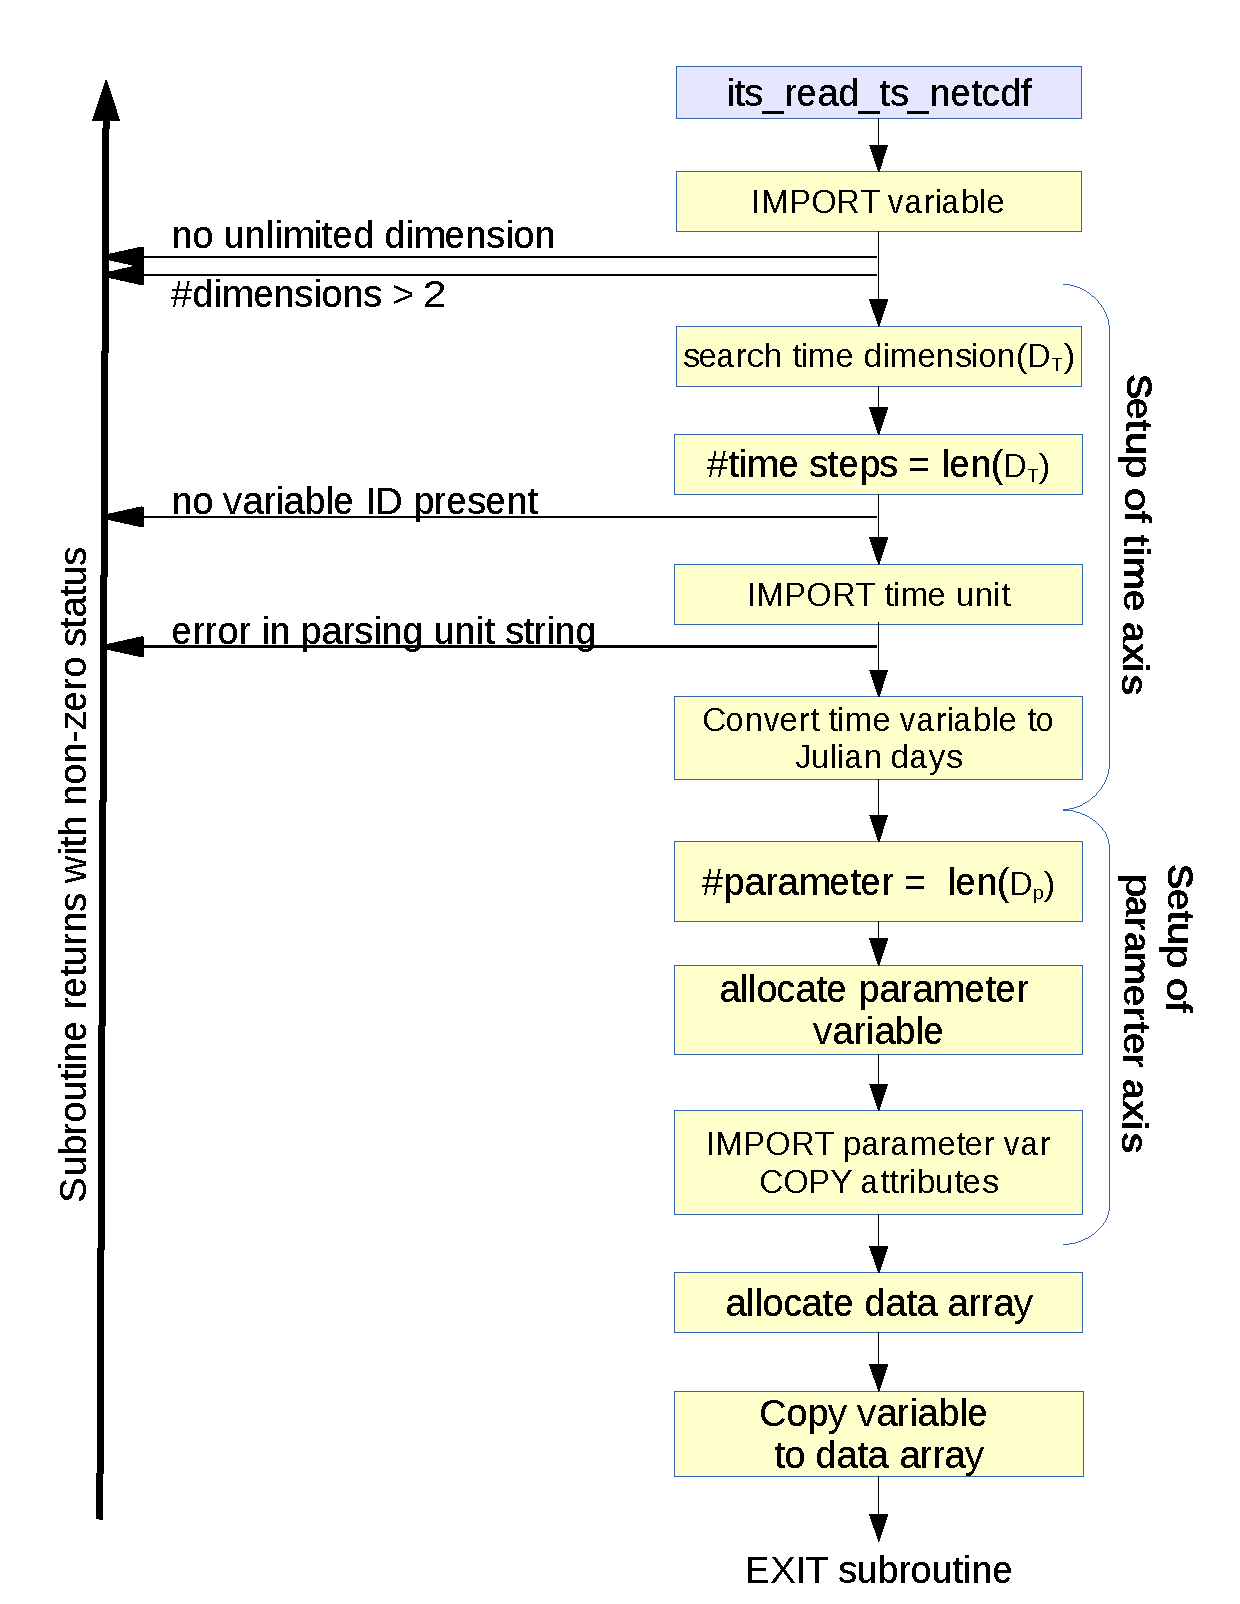
\includegraphics[width=0.7\textwidth]{TS_read_netCDF.pdf}
%\vspace*{.5cm}
\caption{Schematic overview of the data processing in the subroutine
{\tt its\_read\_ts\_netcdf}\label{fig:TSreadnetcdf}.}
\end{figure}
Figure \ref{fig:TSreadnetcdf} schematically illustrates the steps
required in the subroutine to dimension and import the requested data correctly.
More explicitly, the following steps are conducted in the given order: 
\begin{itemize}
\item The two strings are written to the logfile output telling the name of
 the variable to be read and the file from which the variable is read.
\item The local structure \verb|var| of type \verb|T_NCVAR| is read from 
the netCDF file using the subroutine
\verb|IMPORT_NCVAR|, which is provided by MESSy submodel GRID.
 \item If the structure does not contain an unlimited dimension, the
 routine returns with a non-zero error status, as it is required that
 the variable has a time component. 
\item If the number of dimensions of the variable is larger than 2,
 the routine exists with the non-zero error status, 
 because IMORT\_TS only deals with 2D data 
(i.e., time axis x parameter axis).
\item  If no variable ID is 
available, the required information is not accessible from the file and thus
the subroutine returns with a non-zero error status.
\item {\bf Time axis setup:}
\begin{itemize}
\item \underline{Determination of the number of time steps}: A loop over the
dimensions is performed to search for the time dimension (indicated by
the UNLIMITED ID in netCDF). 
If this dimension is found, the length of this
dimension is equal to the number of time steps and thus saved in \verb|zts%nt|
and written to the logfile.
\item \underline{Layout of the time axis}: The respective time
attributes are imported using the subroutine 
\verb|IMPORT_NCATT| (hosted by \verb|messy_main_grid_netcdf.f90|).
The time unit is first written to the logfile and afterwards parsed by the 
subroutine \verb|eval_time_str| (hosted by \verb|messy_main_timer.f90|)
in order to acquire date and time information from the string\footnote{If the string is not successfully parsed, the subroutine returns with an error
status.}
The time variable is read and converted to the julian day format
using the conversion factor and offset determined by the analysis of the netCDF
date string and unit\footnote{The usual netCDF date format is
something like ``hour since 2000-08-01 00:00:00''. From this the unit
(``hours'') and the starting date and time (``2000-08-01 00:00:00'') 
are used to calculate the conversion factors for the internal date
format julian days. Thus a conversion factor for the time unit (here ``hours''
to ``days'') is required (i.e., 24). The offset between the start date
and time (``2000-08-01 00:00:00'') and the 0th julian day is calculated.}.
\end{itemize}
\item {\bf Parameter axis setup}
\begin{itemize}
\item The length of the parameter axis (\verb|zts%np|) is given by the
length of the  
second available dimension. The number of parameters is written to the logfile.
Knowing the number of parameters the component \verb|zts%par| is allocated to 
the correct length and preset with a running index.
\item If the parameter axis is present\footnote{In case of a scalar
variable it is not present.}, the variable is imported
using \verb|IMPORT_NCVAR| and copied to  \verb|zts%par|. 
\item The name of the dimension is copied to
\verb|zts%dimname| and 
\item if dimension attributes exist, these are also copied
to the respective structure component (\verb|zts%dimvaratt|) using 
\verb|COPY_NCATT| (available in the module \verb|MESSY_MAIN_GRID_NETCDF|).
\item The content of  \verb|zts%par| is dumped to the logfile.
\end{itemize}

\item Finally, the structure component hosting the data
(\verb|zts%data|) is allocated and the 
content of the local structure \verb|var| is copied to the structure
describing the data set.
\end{itemize}

 Before leaving the subroutine, the local structure \verb|var| is reinitialised
 and the status flag is set to zero, indicating success of the
 subroutine.

\paragraph{SUBROUTINE \color{blue} \tt\bf its\_read\_ts\_ascii\label{ITSreadasc}\\}
This subroutine is called, if an ASCII file is processed. Parameters of the
subroutine are 
\begin{itemize}
\item a status flag and 
\item the structure \verb|zts| of type \verb|T_TS|.
\end{itemize}

\begin{figure}
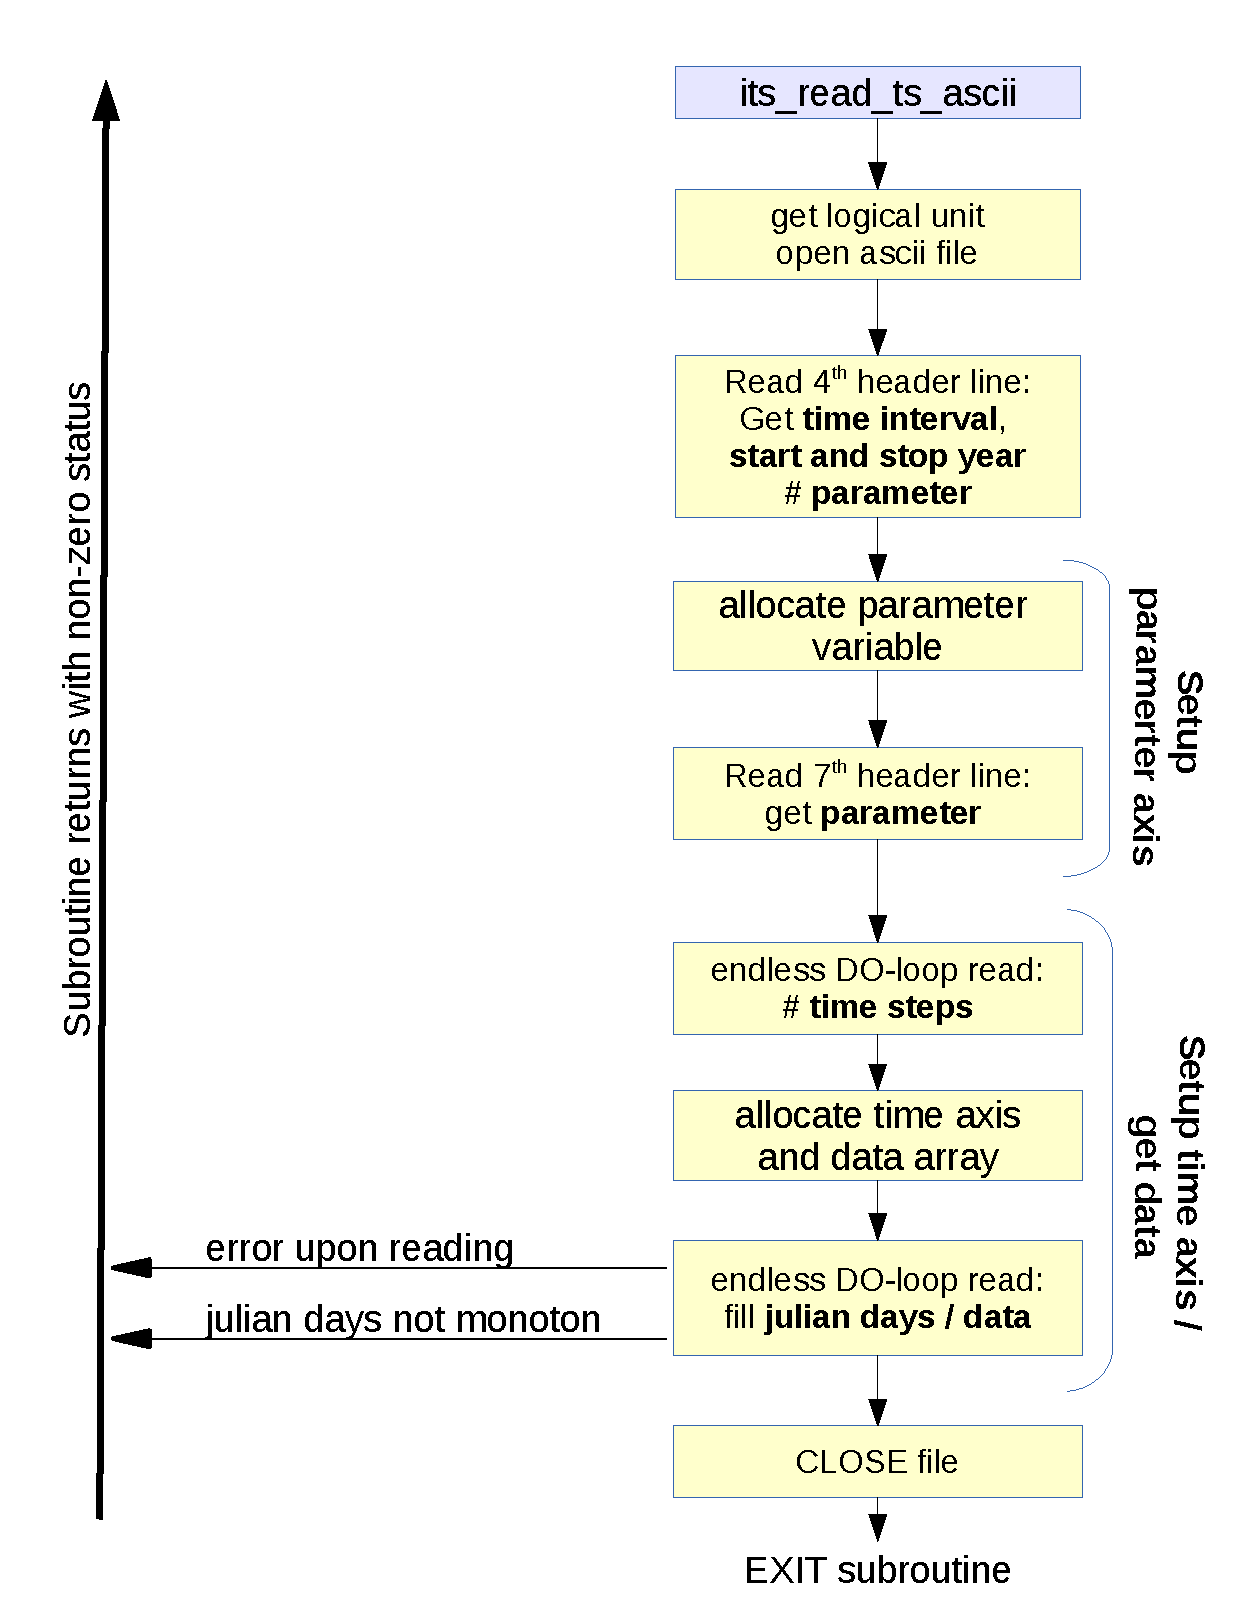
\includegraphics[width=0.7\textwidth]{TS_read_ASCII.pdf}
%\vspace*{-4.5cm}
\caption{Schematic overview of the data processing in the subroutine
{\tt its\_read\_ts\_ascii}\label{fig:TSreadascii}.}
\end{figure}
Figure \ref{fig:TSreadascii} schematically illustrates  the steps
required in the subroutine to dimension and import the requested data
correctly. The subroutine analyses the ASCII
file in the following order: 
\begin{itemize}
\item First it is checked, if the structure
components \verb|zts%jd|, \verb|zts%par| 
and \verb|zts%data| are associated. If so, they are deallocated. Afterwards
all three pointers are NULLIFYied.
\item After acquiring a free unit using the
subroutine \verb|FIND_NEXT_FREE_UNIT|   
from \verb|MESSY_MAIN_TOOLS| the file is opened and the first four
header lines are read and ignored. 
\item From the fifth line the 4 integers 
time interval flag (\verb|flag|), start year (\verb|y1|), end year (\verb|y2|)
and number of parameters (\verb|zts%np|) are read.
If \verb|flag| is outside of the range  1 to 6,
 the subroutine returns with a non-zreo status.
Subsequently, the logfile output, providing the time resolution and
the number of parameters is produced.

\item \underline{Parameter axis setup}:
\begin{itemize}
\item Knowing the number of parameters, the float vector containing
the information about the parameters axis is allocated
(\verb|zts%par(zts%np)|). 
\item This structure component is filled with the content of line 7 of the data
file and the respective information is written to the logfile.
\end{itemize}
\item The header lines 6 and 8 are read, but their content is ignored.

\item \underline{Determination of the number of time steps}: An
endless DO-loop is performed, reading one line (i.e. one time step) 
of the file and enhancing the number of time steps by 1, if the status upon
reading is zero. For a negativ status the DO-loop is existed and thus the 
number of time steps in the file is determined. This information is also
written into the logfile. Afterwards, the file is closed.
\item Knowing the number of time steps, the structure components
containing the julian date  
(\verb|zts%jd|) and the data (\verb|zts%data|) are allocated.

\item \underline{Data acquisition:} To fill the structure components,
 the data file is opened again. The 8 header lines are skipped.
Subsequently, each data line (date (i)) is processed individually.
Depending on the time interval, the 
respective number of integers (e.g., yearly data = 1 integer; daily data = 4
integers) and the data for this specific point in time are read.
If an error occurs upon reading, the subroutine returns with a
non-zero status.
Using the date components, the julian date (\verb|zts%jd(i)|) is calculated 
from the newly read date components. If the julian date does not increase
monotonically within the file, the subroutine returns with a non-zero
status.

\item  Finally, the data file is closed and the status flag is set to zero.
\end{itemize}

\subsubsection{\color{blue} \tt\bf its\_copy\_io\label{ITScopy}}
The subroutine \verb|its_copy_io| copies one structure of
 type \verb|T_TS_IO| to a second structure of the same type. Therefore it
 has two parameters of type \verb|T_TS_IO|.
\begin{verbatim}
  ! -------------------------------------------------------------------
  SUBROUTINE its_copy_io(d, s)

    IMPLICIT NONE

    ! I/O
    TYPE (T_TS_IO), INTENT(OUT) :: d
    TYPE (T_TS_IO), INTENT(IN)  :: s
  ! -------------------------------------------------------------------
\end{verbatim}
The first parameter is the destination structure, the second the
source structure.
Within the subroutine the components of the structure
\verb|T_TS_IO| are copied from the source to the destination.
This subroutine is used to fill the \verb|T_TS_IO| structure component of the
structure of type \verb|T_TS| with the namelist content.

\subsubsection{\color{blue} \tt\bf its\_set\_value\_ts\label{ITSvalue}}
This subroutine performs the data acquisition for the current date.
\begin{verbatim}
  ! -------------------------------------------------------------------
  SUBROUTINE its_set_value_ts(status, zts, yr, mo, dy, hr, mi, se)

    USE messy_main_timer,        ONLY: gregor2julian

    IMPLICIT NONE
    INTRINSIC :: TRIM

    ! I/O
    INTEGER,    INTENT(OUT)   :: status
    TYPE(T_TS), INTENT(INOUT) :: zts
    INTEGER,    INTENT(IN)    :: yr, mo, dy, hr, mi, se
  ! -------------------------------------------------------------------
\end{verbatim}

The arguments of this subroutine are:\\

\begin{tabular}{lllp{6cm}}\hline
 variable & data type &  INTENT & meaning\\\hline
 status &   INTEGER   &  OUT    & error flag (zero = success)\\
 zts    &   TYPE(T\_TS) & IN    & data structure of specific time series\\
 yr     &   INTEGER     & IN    & year of actual simulation time step\\
 mo     &   INTEGER     & IN    & month of actual simulation time step\\
 dy     &   INTEGER     & IN    & day of actual simulation time step\\
 hr     &   INTEGER     & IN    & hour of actual simulation time step\\
 mi     &   INTEGER     & IN    & minute of actual simulation time step\\
 se     &   INTEGER     & IN    & second of actual simulation time step\\\hline
\end{tabular}

The subroutine works as follows:
\begin{enumerate}
\item Calculation of the ``processing date'' / time step to be selected:\\
First, the internal data time components are preset with the simulation
date and time. Afterwards, the date components ``picked'' in the namelist are 
overwritten. This modified date components are converted to julian days,
which is the time format the subroutine is internally working with. This date
is named the ``processing date'' in the following.
\item Date check:\\
First, it is checked whether the processing date lies within the time range
covered by the data file. If not and the ``out of time range'' policy
``0'' is requested, the subroutine returns with a non-zero status.
\item Search for the correct time step:\\
In a DO-loop over all time steps of the data set, the time step \verb|nt| is
searched for  which the processing data lies within the interval 
 \verb|zts%jd(nt)| and \verb|zts%jd(nt+1)|.
\item Data processing and check of data range:\\
The data handling depends on the chosen interpolation method and on whether
the processing date is covered by the data set:
\begin{itemize}
\item If the date is outside the covered time range, but the simulation is
continued, the output object \verb|zts%obj| is
set to the values of the nearest data point, i.e., the first or the last 
time step depending on whether the current date is prior or after the
date range of the data set.
 According to the range of valid data regulated in the namelist, a flag 
(\verb|zts%flg(np)|) is set, indicating whether the data is valid or not.
0 stands for out of range, 1 for valid data.
\item Interpolation method: -1 (previous time step)\\
If interpolation method \verb|-1| was chosen in the namelist, the output object
 \verb|zts%obj|
 is set to the content of the data set at time step \verb|nt|.
Afterwards each entry \verb|np| of the parameter axis is checked, if the data
 is in the valid data range and the flag \verb|zts%flg(np)| is set
accordingly (0 for out of range and 1 for valid data).

\item Interpolation method: 0 (linear interpolation between previous
 and next time step)\\ 
If linear interpolation between the two nearest points in time is requested,
a weighting factor \verb|f| depending on the distance to the two adjacent points in time
is calculated and the output data is then weighted between these two points
in time according to this factor:
\begin{verbatim}
f = (jd - zts%jd(nt)) / (zts%jd(nt+1) - zts%jd(nt))
zts%obj(:) = f * zts%data(nt+1,:) + (1.0 - f) * zts%data(nt,:)
\end{verbatim}
In contrast to the two other interpolation methods, it is checked, 
whether the data of both times of the original data set are within the
required range and the flag \verb|zts%flg(np)| is set accordingly.

\item Interpolation method: ~1 (next time step)\\
If interpolation method \verb|1| was chosen in the namelist, the output object
 \verb|zts%obj| is set to the content of the data set at time step \verb|nt+1|.
Afterwards each entry \verb|np| of the parameter axis is checked, if the data
 is in the valid data range and the flag \verb|zts%flg(np)| is set
accordingly (0 for out of range and 1 for valid data).
\end{itemize}
\end{enumerate}
Finally the status flag is set to 0 indicating the success of the subroutine
upon return to the calling routine.

\subsubsection{\color{blue} \tt\bf its\_delete\_ts\label{ITSdelete}}
Within the subroutine \verb|its_delete_ts| the components of a structure
of type \verb|T_TS| are deallocated or, depending on the data type,
 set to their initial values, respectively.

%*************************************************************************
\subsection{The Basemodel Interface Layer}
%*************************************************************************
The BMIL of IMPORT\_TS uses four MESSy entry points:
\begin{itemize}
\item  two in the initial phase, 
\begin{itemize} 
\item the first for reading and analysing the namelist (\verb|import_ts_initialise|), and
\item the second for memory initialisation (\verb|import_ts_init_memory|),
\end{itemize}
\item one during the integration phase (\verb|import_ts_global_start|), and 
\item the last one in the finalising phase freeing the memory allocated by
 the submodel (\verb|import_ts_free_memory|).
\end{itemize}

\subsubsection{import\_ts\_initialise}
In the first call during the initialisation phase of MESSy, the namelist
\verb|&CTRL_TS| contained in the namelist file \verb|import.nml| is read
and analysed.
For reading the SMCL subroutine  \verb|IMPORT_TS_READ_NML_CTRL| (Sect.~\ref{ITSreadctrl}) is called on the I/O-PE.
Afterwards the namelist entries of type \verb|T_TS_IO| are processed on the I/O-PE. First the algorithm loops over the maximum number of input data sets 
(\verb|NMAXTS|). The algorithm cycles, if the name is empty, as this indicates,
that no event with this number was defined in the namelist.
Otherwise the read structure \verb|TS| of type \verb|T_TS_IO| is copied to
\verb|XTS(NTS)%io| using the SMCL subroutine \verb|its_copy_io|
 (Sect.~\ref{ITScopy}), where \verb|XTS| is of type \verb|T_TS|, \verb|io|
is its component of type \verb|T_TS_IO|, and \verb|NTS| is a running index
for the respective data set.
The namelist entries are written to the logfile
(see Sect.~\ref{ITSBOXrun} for more details). After analysing the namelist
entries, the file is opened and analysed using the SMCL subroutine
\verb|its_read_ts| (Sect.~\ref{ITSread}).
Within this subroutine the other components of the structure \verb|XTS| are
allocated according to the dimensions read from the file.

After all namelist entries have been processed on the I/O-PE, \verb|NTS|
is set to the actual number of namelist entries. First, this number is 
broadcasted to all PEs. In a second loop over all actual data sets, the 
results of the namelist and file analyses are broadcasted to all PEs and
the data arrays are allocated on all PEs.

\subsubsection{import\_ts\_init\_memory}
Here, the memory for the actual output data is allocated in form of channel
objects\footnote{See the Channel User Manual, which is part of the electronic supplement of J\"ockel et al., 2010}.

At the beginning, two list variables \verb|list_dimid|
 and \verb|list_reprid| 
 are dimensioned according to the number of data sets. 
In a loop over all data sets, the following steps are required to
 determine the correct dimensioning of the channel objects for each
 data set.
\begin{enumerate}
\item Determination of the \verb|dimension ID|:\\
the correct dimension ID required for the parameter axis needs to be identified, if it already exists, or created, if it does not yet exist.
Calling the CHANNEL subroutine \verb|get_dimension_info| it is tested, 
whether the dimension ID already exists. If so, the subroutine returns with the
 status flag set to zero and the two variables \verb|DIMID|, providing the 
respective dimension ID, and \verb|len|
providing the length of the dimension. If  \verb|len| is not 
identical to the number of parameters for the respective data set, the dimension
name exists already, but not with the correct length. Therefore the dimension
name needs to be changed. In this case an arbitrary number between 1 and 1000
is added to the name. In a loop from 1 to 1000 a dimension name is searched,
which does not already exist.
If an unused dimension name is found, the number is added to the original
dimension name

\verb|XTS(i)%dimname = TRIM(XTS(i)%dimname)//nrstr|

with \verb|nrstr| the added number as string, and the logical identifier 
\verb|ldim_ok| is set to \verb|.TRUE.|.
\verb|ldim_ok = .TRUE.| indicates, that the dimension needs to be created,
while  \verb|ldim_ok = .FALSE.| means, that a dimension of the correct 
length exists.
If \verb|ldim_ok = .TRUE.| a new dimension of the length of the
parameter axis (\verb|XTS(i)%np|) and the name determined above is defined.
The corresponding dimension variable is filled with the float values of 
\verb|XTS(i)%par| (i.e., the content of line 7 in an ASCII file).
Additionally, if dimension attributes are defined in the input file
(netCDF file only), they are copied as attributes to the dimension variable.
The dimension ID of the newly defined dimension is saved in the variable
\verb|list_dimid|. For  \verb|ldim_ok = .FALSE.| the dimension ID of the
already existing dimension is saved in \verb|list_dimid|.

 \item Definition of the \verb|representation|:\\
After the dimension is determined, the representation of the channel object
needs to be acquired. First it is checked, if the dimension ID of the
current data set was already used for a previous data set. In this case,
the same representation can be used.
If this is not the case, a new representation for a 1D variable on an
 ``N''-axis is defined. All respresentation names defined by
 IMPORT\_TS start with 
the string ``TSR\_''. 
The representation ID of the newly defined representation is saved in the
variable \verb|list_reprid|.
\item Definition of the data channel object: \\
Finally, the new channel object and its attributes are defined.
The channel is named \verb|import_ts| and the variable name from the
namelist is used as channel object name. 
The information provided by the original namelist entry are defined as 
namelist attributes for the channel object, i.e., the filename, the valid range,
the ``out of to time range'' policy and the interpolation method.

\item Definiton of the ``flag'' channel object:\\
 A second channel object with the same representation is defined, which contains
the flag indicating whether the data is in the valid range 
(\verb|XTS(i)%flag = 1|) or not (\verb|XTS(i)%flag = 0|).
\end{enumerate}

\subsubsection{import\_ts\_global\_start}
This subroutine is called at the beginning of the time loop.
Looping over all data sets,  the time series data is processed according to the 
 actual simulation date using the SMCL subroutine \verb|its_set_value_ts|.
\subsubsection{import\_ts\_free\_memory}
At the end of the integration the allocated memory (for the
variables \verb|list_dimid| and \verb|list_reprid|) is released. 

%*************************************************************************
%*************************************************************************
\section{The stand-alone tool IMPORT\_TS\label{ITSBOX}}
The stand-alone tool of IMPORT\_TS is part of the electronical supplement
as this User Manual. 

\subsection{Installing stand-alone tool IMPORT\_TS}
\begin{enumerate}
\item unzip the zip-file:\\
\verb|unzip import_ts.zip|
\item change into the subdirectory \verb|./import_ts|:\\
\verb|cd import_ts|
\item add the necessary entries for your system and compiler to the \verb|Makefile|, i.e.,

\begin{tabular}{lp{12cm}}
 \verb|F90| & Fortran90/95 compiler \\
 \verb|F90FLAGS| & Fortran90/95 compiler options (e.g., options for invoking the cpp preprocessor \\
 \verb|DEFOPT| &  prefix for compiler directive definitions \\
\verb|NETCDF_LIB| & netCDF library path \\
\verb|NETCDF_INCLUDE| & netCDF include path\\
\end{tabular}

\item build the executables and modules:\\
\verb|gmake|

\item the directory can be cleaned by\\
\verb|gmake clean|
\end{enumerate}
The executable \verb|import_ts.exe| should now be available in the  
 main directory. 
The status after unpacking the zip-file can be archieved with
\verb|gmake distclean|.

\subsection{Running the stand-alone tool IMPORT\_TS\label{ITSBOXrun}}
After setting up IMPORT\_TS as described in the previous section, IMPORT\_TS
is run by 
\begin{verbatim}
./import_ts.exe import.nml
\end{verbatim}

The \verb|import.nml| namelist file should contain at least one entry in the
\verb|&CTRL_TS| namelist.
An example file is distributed together within the stand-alone tool.

The tool produces the following logfile output:
\begin{verbatim}
**************************************************************************
 *** START import: INITIALISATION (import_ts_read_nml_ctrl)
 Reading namelist 'CTRL_TS' from 'import.nml' (unit  101 ) ...
  ... OK !
 *** END   import: INITIALISATION (import_ts_read_nml_ctrl)
 **************************************************************************
 TIME SERIES   : test
    FILE       : test_data_monthly.txt
    VALID RANGE:  -99.9000000000000057 99.9000000000000057
    BND POLICY : stop
    BND POLICY : stop
    SELECTION  : linear interpolation
    READING DATA ...
     its_read_ts_ascii: OPENING FILE test_data_monthly.txt
     its_read_ts_ascii: TIME RESOLUTION      : month 
     its_read_ts_ascii: NUMBER OF PARAMETERES:  19
     its_read_ts_ascii: AXIS                 :  300.000000000000000 
        400.000000000000000 500.000000000000000 600.000000000000000
        800.000000000000000 1000.00000000000000 1200.00000000000000
        1500.00000000000000 2000.00000000000000 2500.00000000000000 
        3000.00000000000000 3500.00000000000000 4000.00000000000000 
        4500.00000000000000 5000.00000000000000 6000.00000000000000 
        7000.00000000000000 8000.00000000000000 9000.00000000000000
     its_read_ts_ascii: NUMBER OF TIME STEPS :  642
     its_read_ts_ascii: CLOSING FILE test_data_monthly.txt
     its_read_ts: RANGE OF JULIAN DAY  :  2434743.50000000000  -  2454252.50000000000
     its_read_ts: RANGE OF DATA        :  -41.0000000000000000  -  99.9000000000000057
     its_read_ts: PICK OUT             :  -1 -1 -1 -1 -1 -1
     its_read_ts: OFFSET               :  0.000000000000000000E+00  days
    ... DONE!
 ------------------------------------------------------
 ======================================================
 TIME INTEGRATION STARTS ...
  ... DONE!
 ======================================================
\end{verbatim}
First, the \verb|&CTRL_TS| namelist is read without error. Afterwards the
tool loops over all possible \verb|TS| events and produces
analytical output. 
In the example, only one event is found. Its name is 'test' and the file
``\verb|test_data_monthly.txt|'' is read. The valid data ranges between
-$90.0$ and $90.0$. The simulation is stopped, if the simulation date is outside
the time span covered by the data file. The data will be linearly
interpolated 
for dates between two data points in the file.
Subsequently, the header lines are evaluated: The file contains monthly data.
 The parameter axis is 19 entries long. The respective values (here
 heights) are listed in the line labeled AXIS. 
After the evaluation of the header, the data set is scanned:
It is 642 steps long, ranges from julian day  2434743.50 to julian day 
 2454252.50. The actual range of data is -41.0 to 99.90. No special day is
picked and no offset was requested.
After the initial phase, the time integration starts. In this case,
the model loops from the start date of the data file to the end date and
processes the data for all parameters and dates as requested in the namelist.
 The result is written
into an ASCII output file named \verb|output_xx.dat|, where \verb|xx| is a
place holder for the index of the processed time series data set. 

%% \subsubsection{File conversion}
%% In special cases it might be easier to edit an ASCII fileconvert the easier editable ASCII file
%% to a netCDF file in the end. In the box model file a ferret jnl-script named
%% \verb|convert.jnl| can be found, which does exactly the required conversion.
%+++++++++++++++++++++++++++++++++++++++++++++++++++++++++++++++++++++++++++
%+++++++++++++++++++++++++++++++++++++++++++++++++++++++++++++++++++++++++++
%% \begin{appendix}

%% \chapter*{\noindent Glossary}

%% \end{appendix}

%+++++++++++++++++++++++++++++++++++++++++++++++++++++++++++++++++++++++++++
%+++++++++++++++++++++++++++++++++++++++++++++++++++++++++++++++++++++++++++
%+++++++++++++++++++++++++++++++++++++++++++++++++++++++++++++++++++++++++++


\bibliographystyle{copernicus} % bst file
\bibliography{main_import}     % bib files

%%%%%%%%%%%%%%%%%%%%%%%%%%%%%%%%%%%%%%%%%%%%%%%%%%%%%%%%%%%%%%%%%%%%%%%%%
%!!!!!!!!!!!!!!!!!!!!!!!!!!!!!!!!!!!!!!!!!!!!!!!!!!!!!!!!!!!!!!!!!!!!!!!!
%%%%%%%%%%%%%%%%%%%%%%%%%%%%%%%%%%%%%%%%%%%%%%%%%%%%%%%%%%%%%%%%%%%%%%%%%
% subroutines to move? rename?
%%%%%%%%%%%%%%%%%%%%%%%%%%%%%%%%%%%%%%%%%%%%%%%%%%%%%%%%%%%%%%%%%%%%%%%%%
%   main_import_grid_write_restart
%   main_import_grid_read_restart
%   import_grid_free_memory
% all 3 from import_grid_tools_bi to import_grid_bi, as these are the files
% called from CONTROL and basemodel directly. These should not be in the
% ``subsub-part'', but in the main interface file
% also the names does not include tools
% especially import_grid_free_memory has nothing to do in tools_bi !, 
%
% except, I see that, they all handle the RGEVENTS, which are located in 
% tools, but than we need the call then through import_grid and name the 
% subroutine accordingly, i.e., main_import_grid_tools_free_memory
% main_import_grid_tools_write(read)_restart (thats now my favourite)
%------------------------------------------------------------------------
% &RGEVENTS namelist should be named &IMPORT_GRID consistent to &IMPORT_TS
% as it is the namelist of the submodel IMPORT_GRID
%
%%%%%%%%%%%%%%%%%%%%%%%%%%%%%%%%%%%%%%%%%%%%%%%%%%%%%%%%%%%%%%%%%%%%%%%%%
% renaming necessary for consistency?
%%%%%%%%%%%%%%%%%%%%%%%%%%%%%%%%%%%%%%%%%%%%%%%%%%%%%%%%%%%%%%%%%%%%%%%%%
% RGEVENT RGTEVENT
% RGTEVENT_INIT_ONL  wozu wird diese routine gebraucht?
%
%
%%%%%%%%%%%%%%%%%%%%%%%%%%%%%%%%%%%%%%%%%%%%%%%%%%%%%%%%%%%%%%%%%%%%%%%%%
%!!!!!!!!!!!!!!!!!!!!!!!!!!!!!!!!!!!!!!!!!!!!!!!!!!!!!!!!!!!!!!!!!!!!!!!!
%%%%%%%%%%%%%%%%%%%%%%%%%%%%%%%%%%%%%%%%%%%%%%%%%%%%%%%%%%%%%%%%%%%%%%%%%

\end{document}
